\chapter{Phase 1: Physical Access, Firmware Extraction \& Analysis}
This chapter is dedicated to the technical characterization of the Shelly Plug S (Gen 1), chosen as a case study for security analysis. Before proceeding with vulnerability identification, it is essential to define the system architecture by analyzing both the device's operational capabilities and the hardware configuration of the Printed Circuit Board (PCB). Starting from the description of the factory functionalities, the analysis then delves into the hardware components, identifying the key elements that constitute the physical and logical attack surface of the system. 


\section{Features and Functionality of the Device}
The Shelly Plug S is a smart actuator designed for the remote monitoring and control of domestic electrical loads. It stands out in the IoT scenario due to its small size, which allows it to be used in standard wall sockets without obstructing adjacent plugs.

\noindent The device acts as an interface between the electrical infrastructure and the digital network, enabling not only remote power switching but also the real-time detection of electrical consumption parameters.

\medskip
\noindent From a connectivity perspective, the system operates on the 2.4 GHz band using the Wi-Fi 802.11 b/g/n standard. The firmware architecture includes an integrated web server that allows standalone operation, ensuring full configuration and control within the local network without relying on external cloud infrastructures.

\noindent This structural independence facilitates interoperability with third-party platforms through native support for standard communication protocols such as HTTP, UDP, MQTT, and CoAP.

\medskip
\noindent The local web interface provides an intuitive dashboard to control the relay status, monitor power consumption, and schedule operations. Figure \ref{fig:shelly_web_ui} shows the main page of the integrated web server.

\begin{figure}[H]
    \centering
    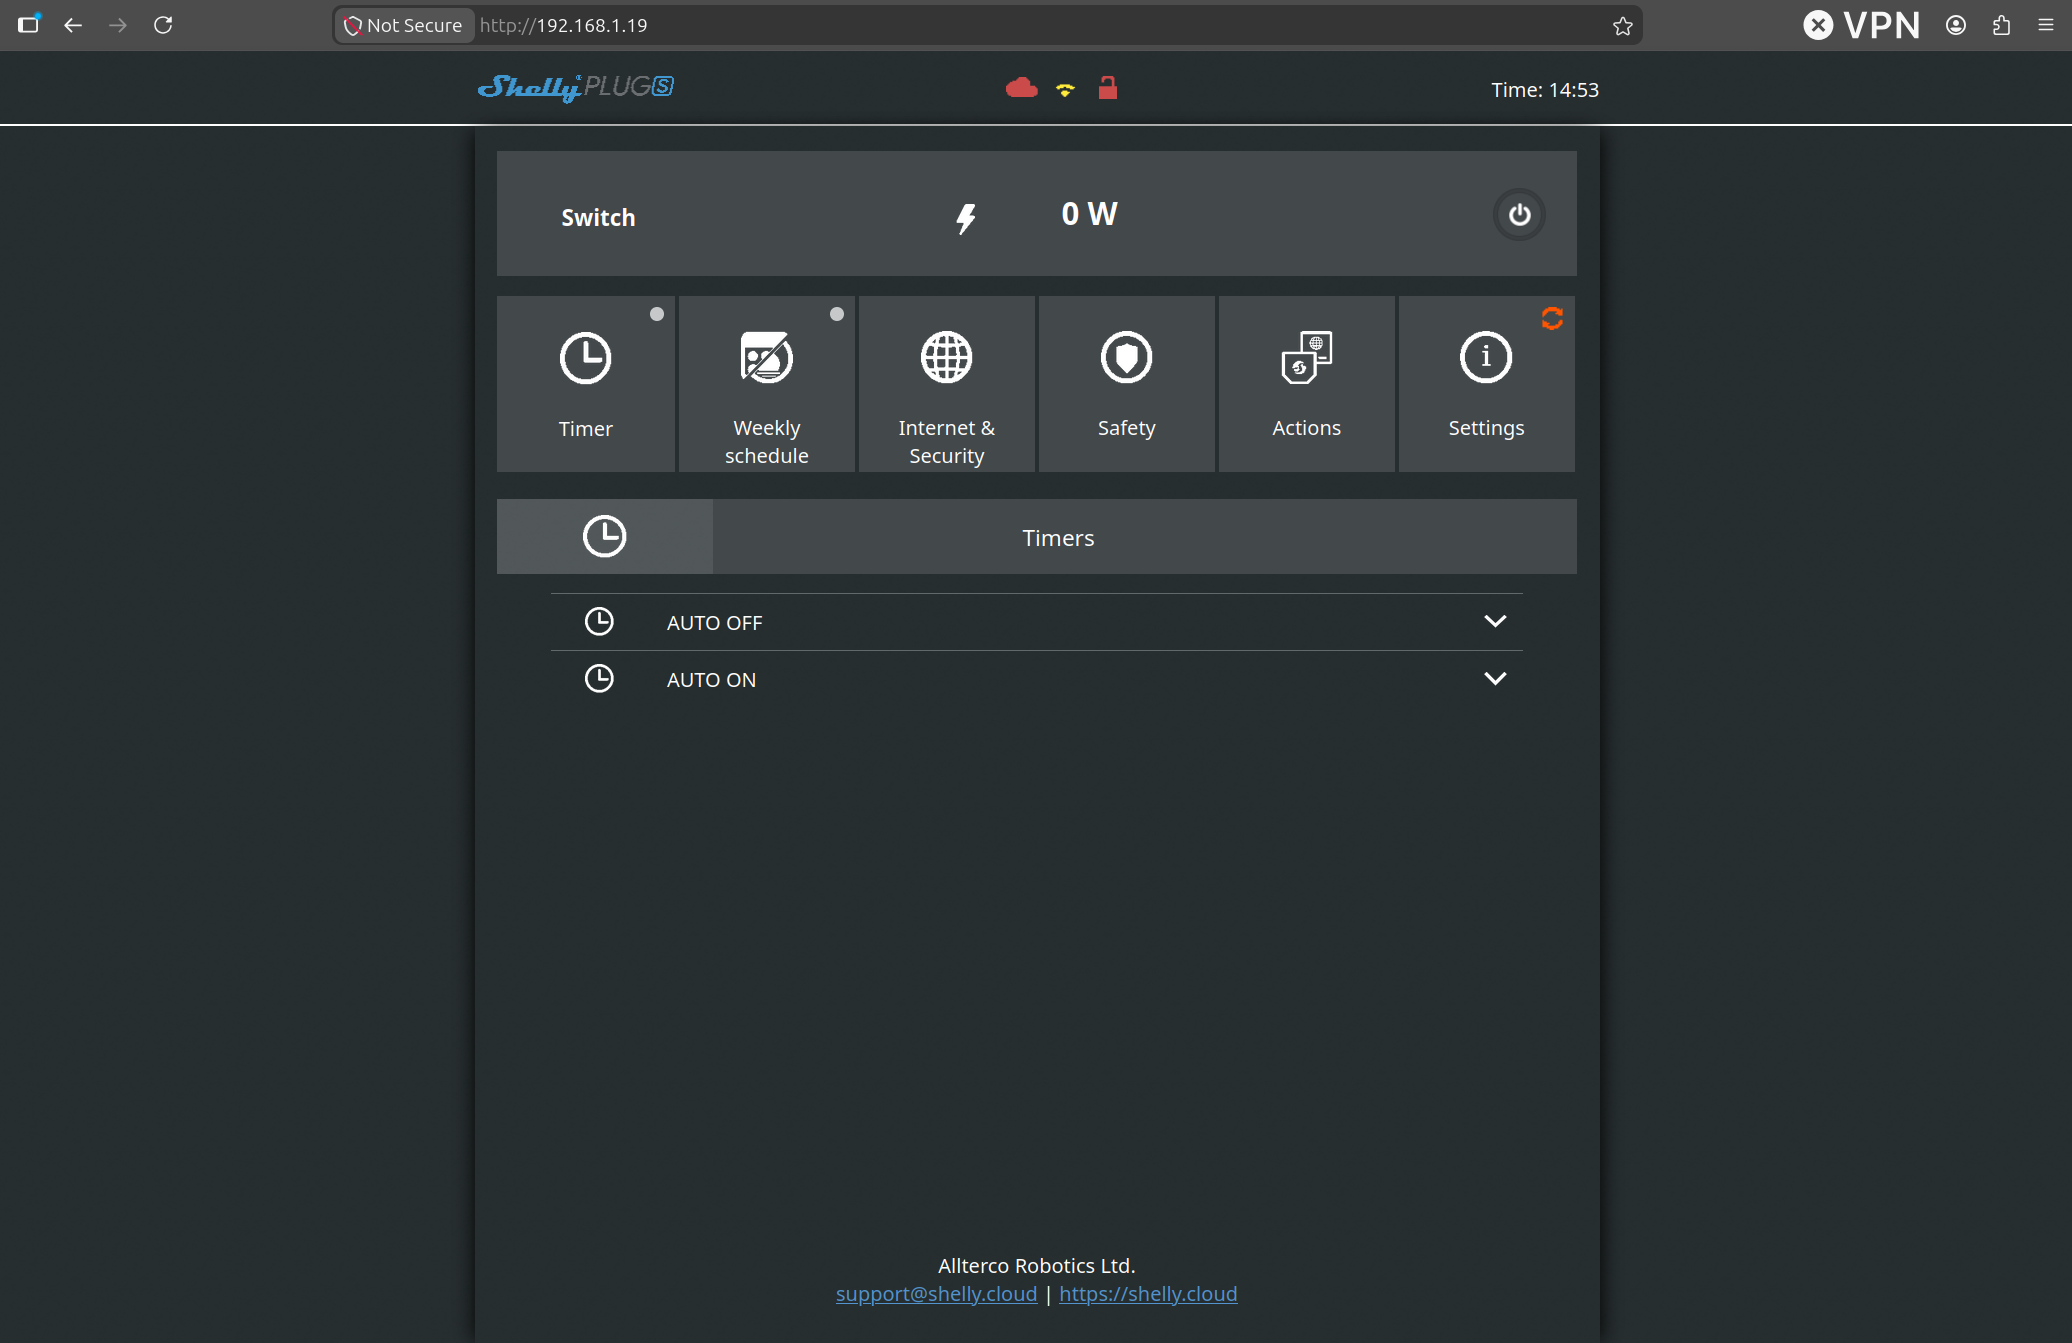
\includegraphics[width=0.85\linewidth]{Images/Fase1/Interfaccia1.png}
    \caption{Shelly Plug S native web interface home page}
    \label{fig:shelly_web_ui}
\end{figure}

\noindent Within this interface, users can also configure automated tasks such as weekly schedules (Figure \ref{fig:shelly_schedule}) and customize safety parameters like the maximum power threshold (Figure \ref{fig:shelly_safety}).

\begin{figure}[H]
    \centering
    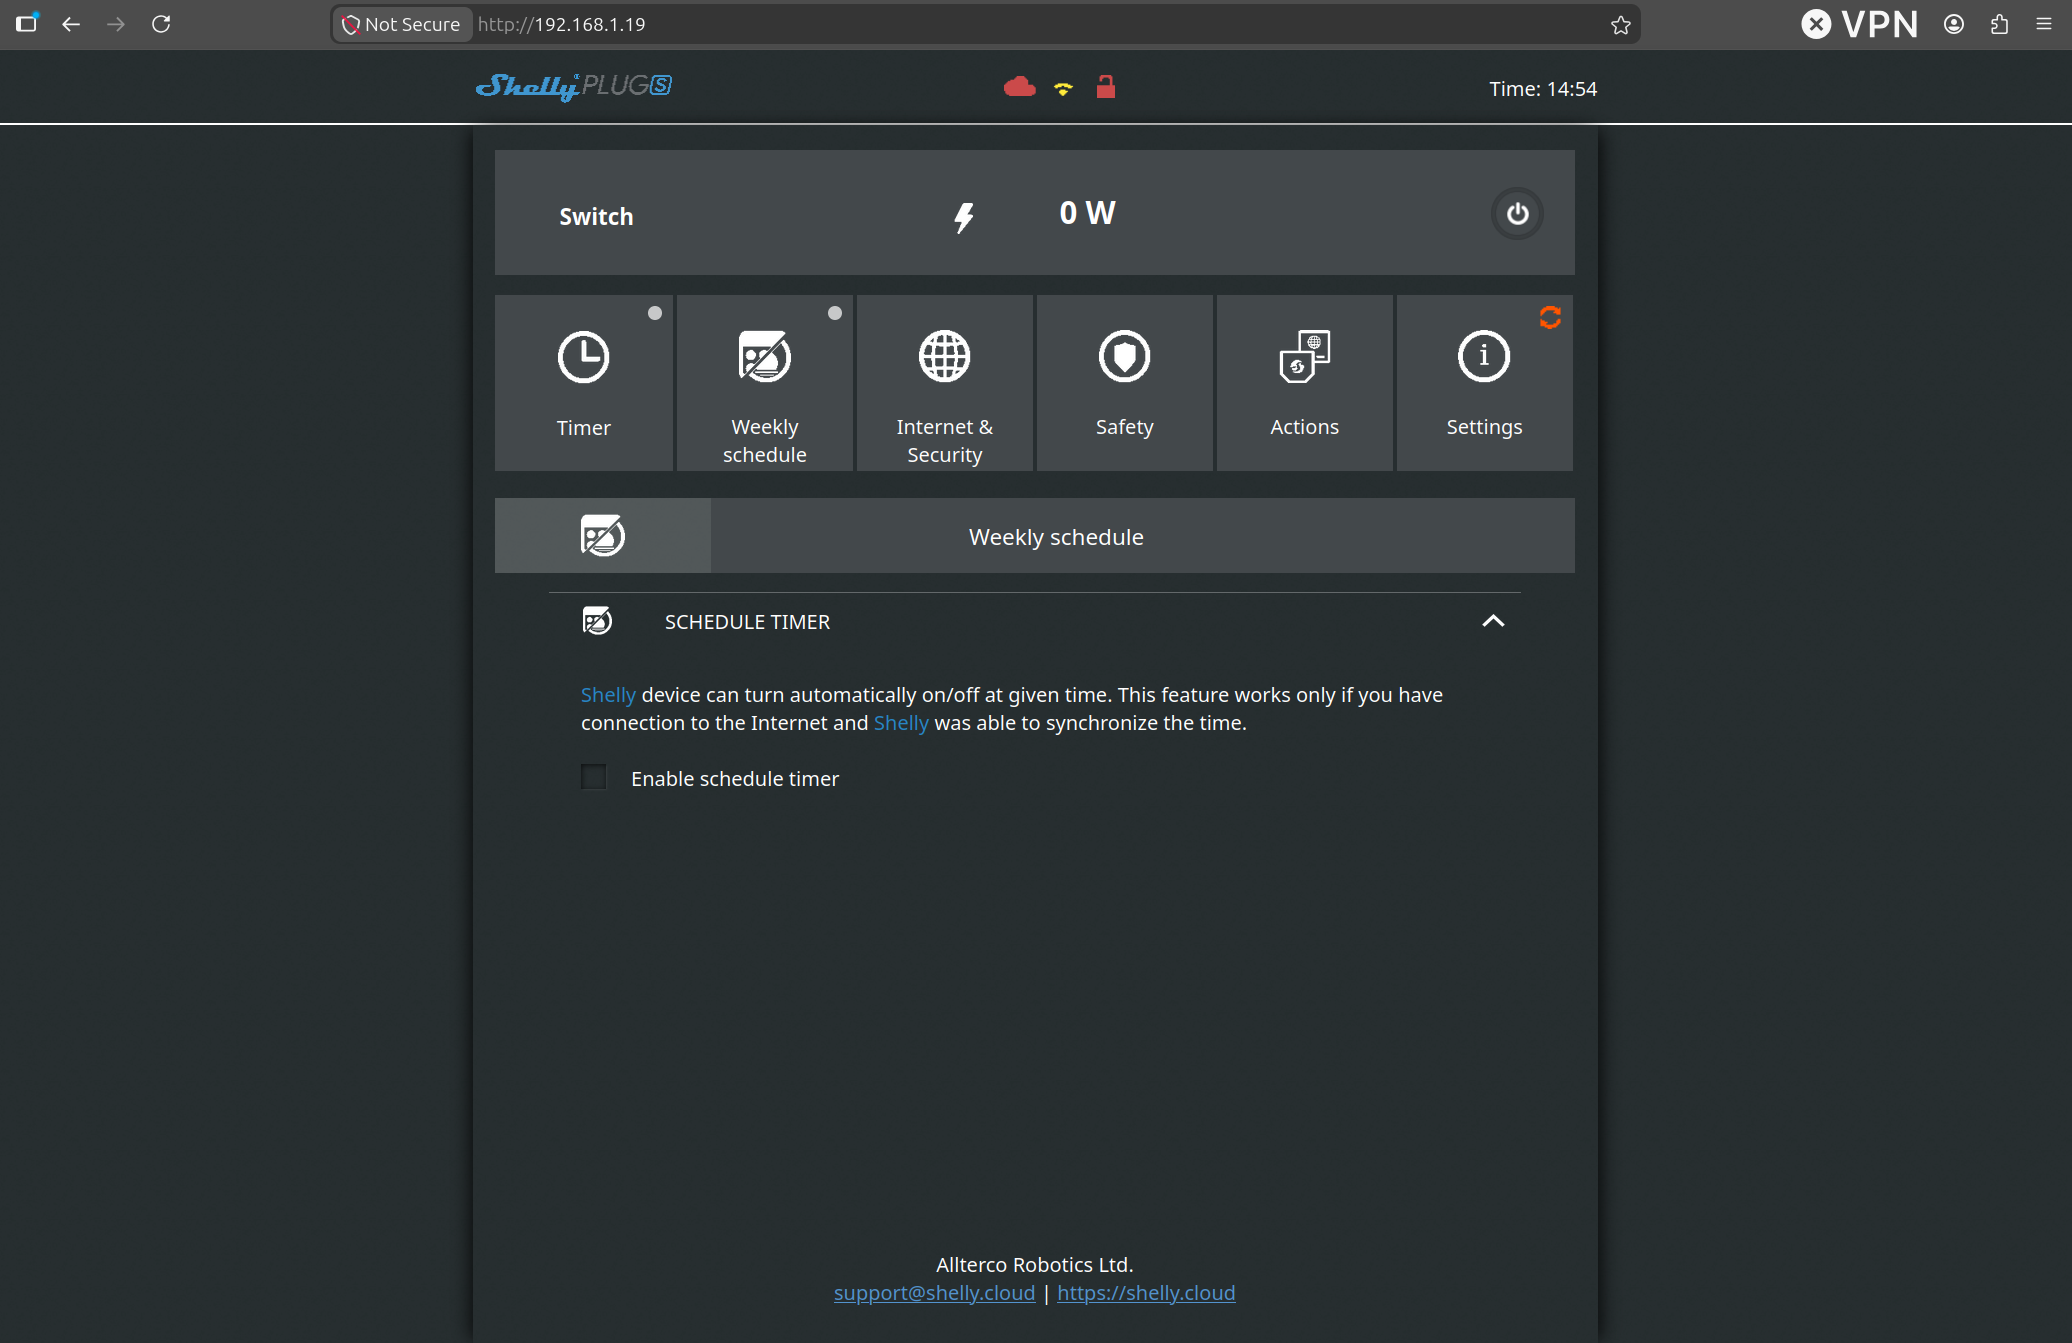
\includegraphics[width=0.8\linewidth]{Images/Fase1/Interfaccia2.png}
    \caption{Weekly schedule configuration page in the local Web UI}
    \label{fig:shelly_schedule}
\end{figure}

\begin{figure}[H]
    \centering
    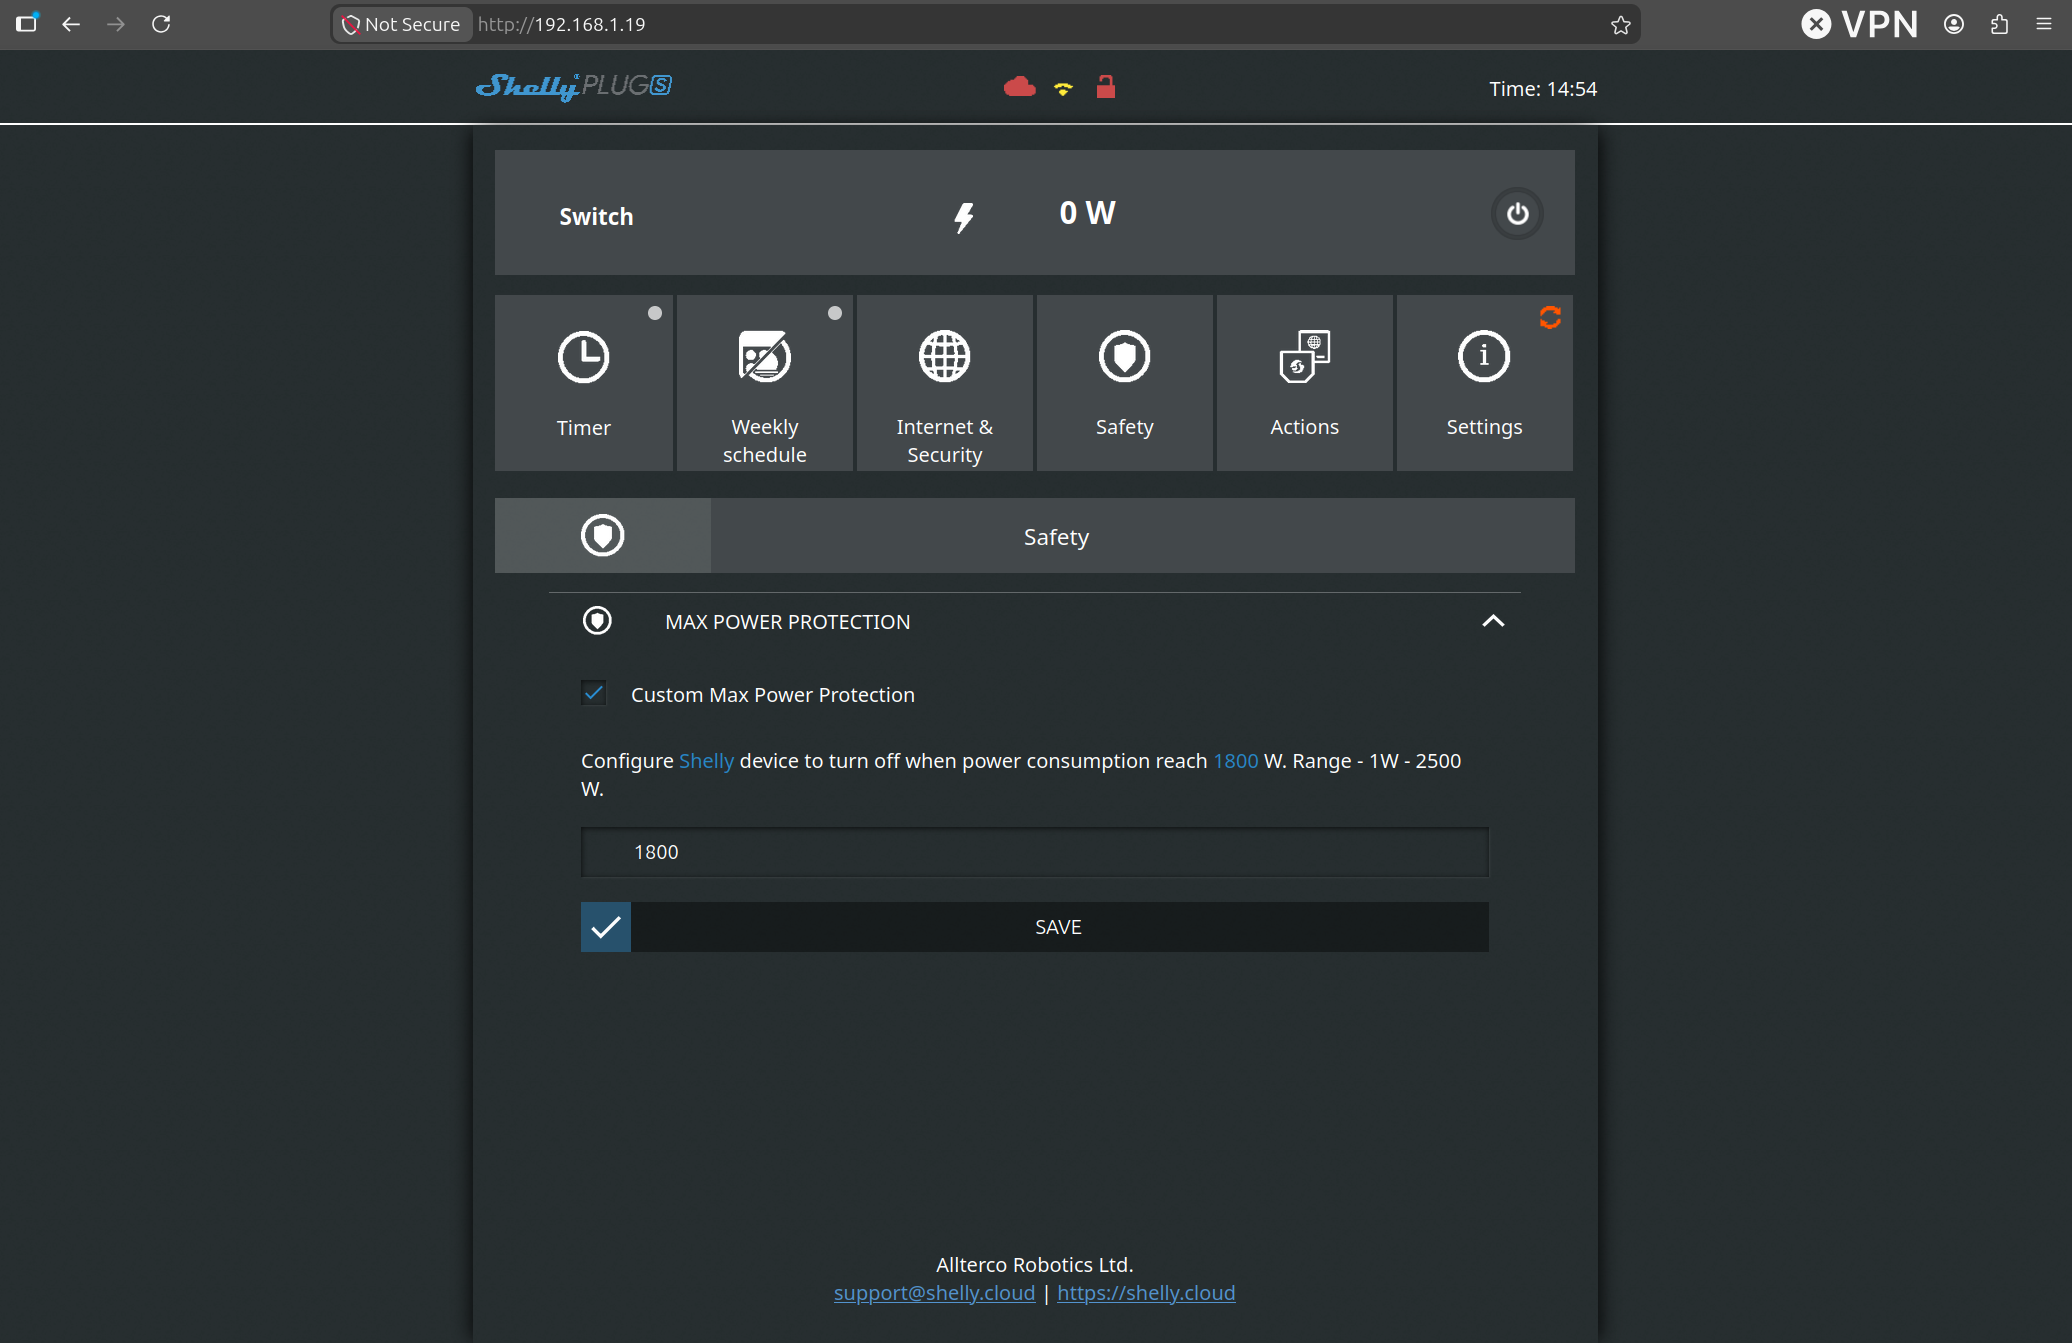
\includegraphics[width=0.8\linewidth]{Images/Fase1/Interfaccia4.png}
    \caption{Max power protection settings in the local Web UI}
    \label{fig:shelly_safety}
\end{figure}

\noindent Furthermore, a dedicated settings menu (Figure \ref{fig:shelly_settings}) allows managing system configurations, including firmware updates, default power-on states, and device reboots.

\begin{figure}[H]
    \centering
    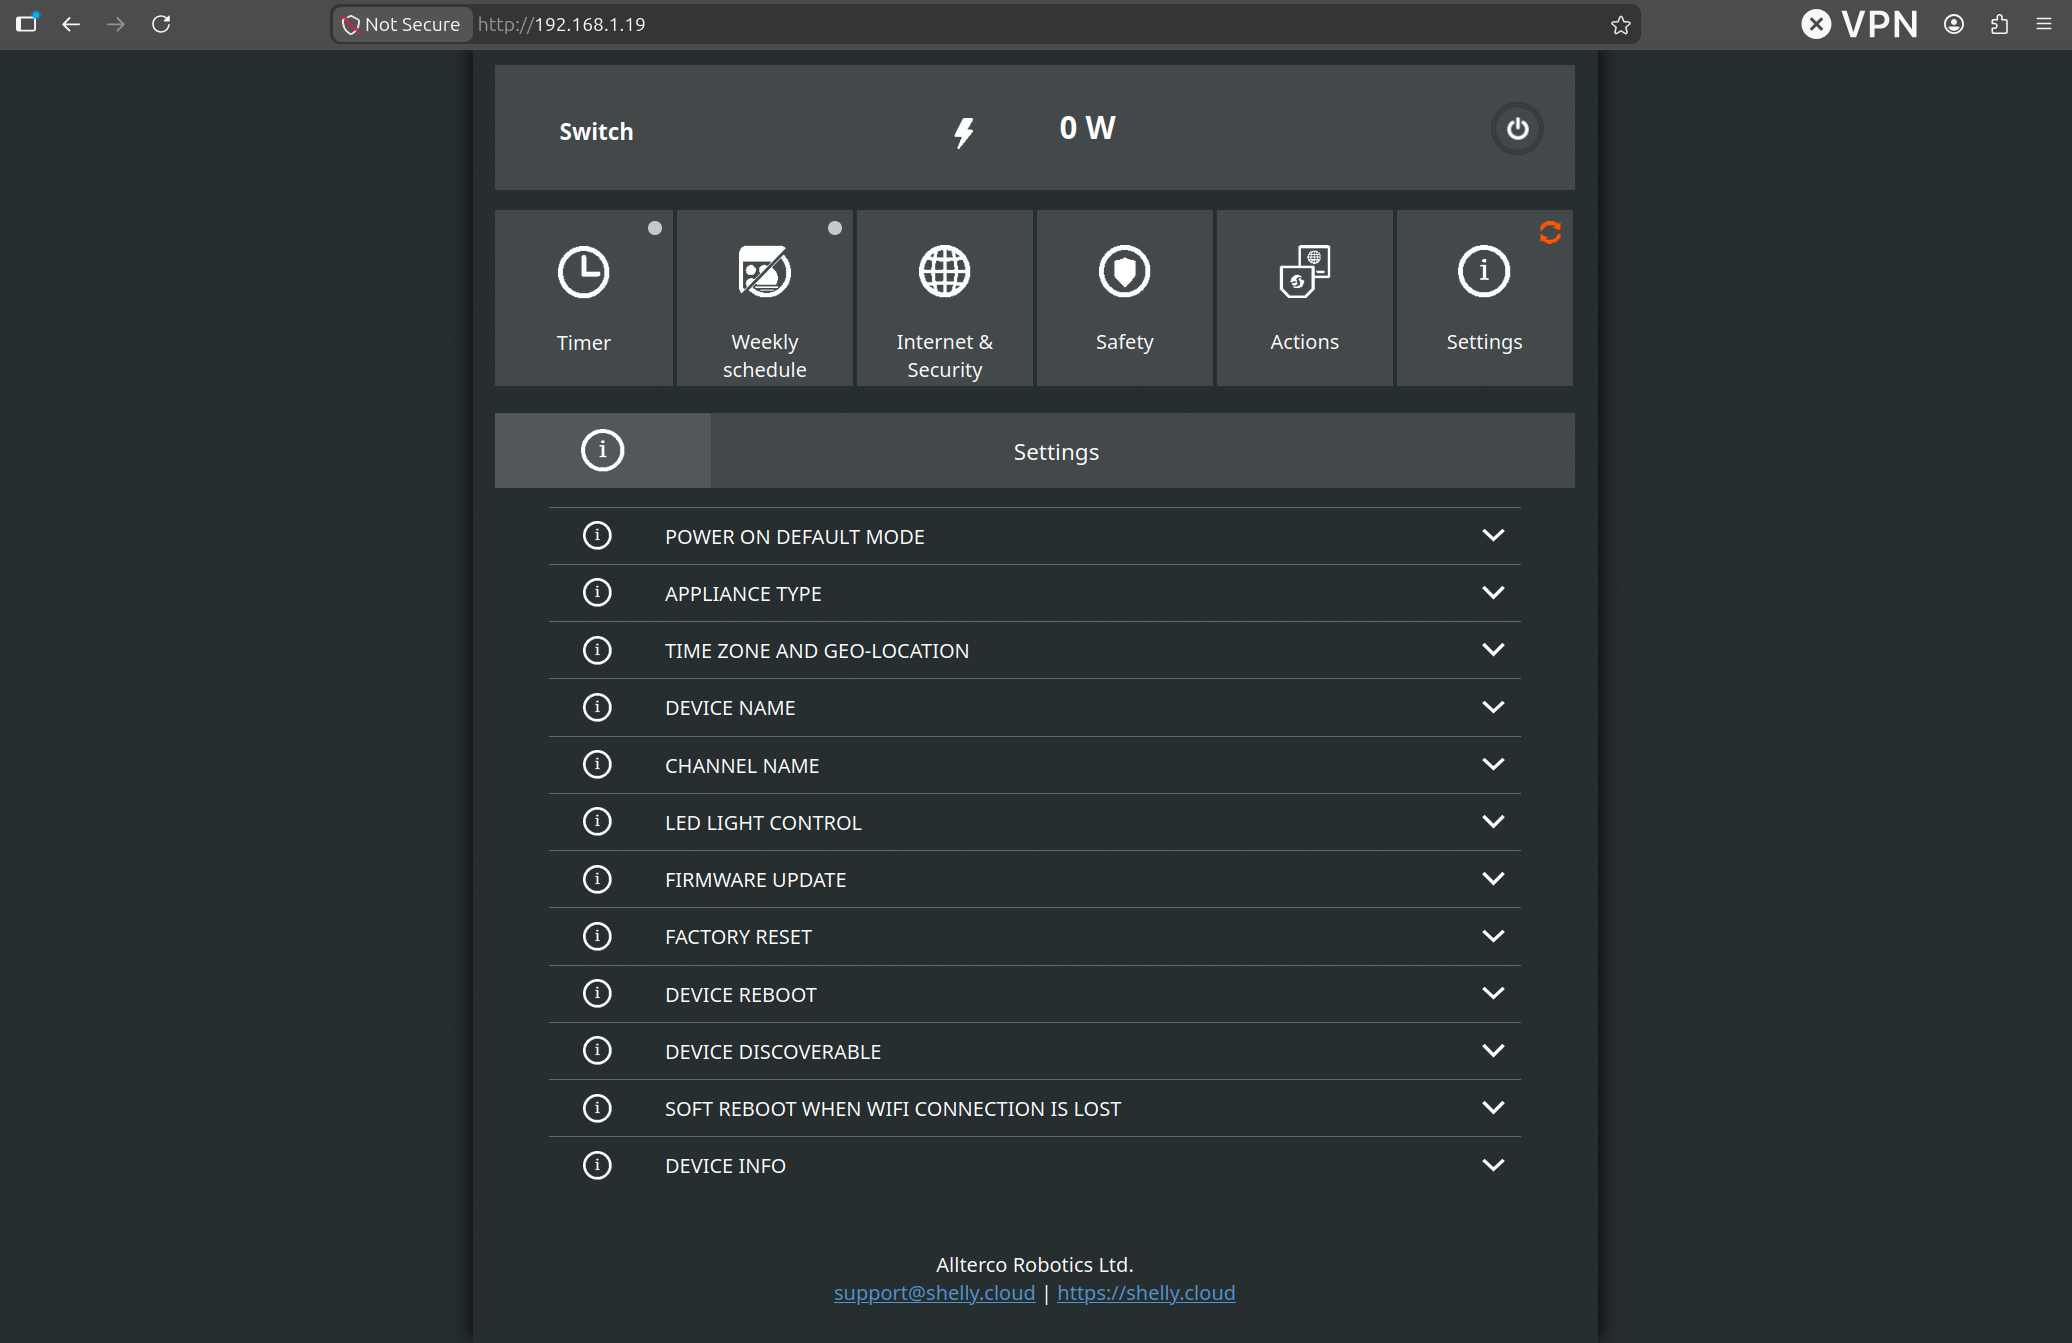
\includegraphics[width=0.8\linewidth]{Images/Fase1/Interfaccia5.png}
    \caption{General settings menu in the local Web UI}
    \label{fig:shelly_settings}
\end{figure}

\medskip
\noindent The main technical specifications provided by the manufacturer are summarized in Table~\ref{tab:technical_specs}:

\begin{table}[H]
    \centering
    \small
    \renewcommand{\arraystretch}{1.3}
    \setlength{\tabcolsep}{12pt}
    \begin{tabular}{ll}
        \toprule
        \textbf{\color{darkblue}Specification Parameter} & \textbf{\color{darkblue}Value / Details} \\
        \midrule
        \rowcolor{lightgray}
        Power Supply & 110--230 V $\pm$10\% 50/60Hz AC \\
        Max Load & 10A / 230V, 50/60Hz \\
        \rowcolor{lightgray}
        Working Temperature & -20°C to 40°C \\
        Radio Signal Power & 1 mW \\
        \rowcolor{lightgray}
        Radio Protocol & Wi-Fi 802.11 b/g/n \\
        Frequency & 2412--2472 MHz (max. 2483.5 MHz) \\
        \rowcolor{lightgray}
        Operational Range & Up to 50 m outdoors / 30 m indoors \\
        Dimensions (HxWxL) & 70x44x44 mm \\
        \rowcolor{lightgray}
        Electrical Consumption & $<$ 1W \\
        SAR & 1.15 W/Kg \\
        \bottomrule
    \end{tabular}
    \caption{Official technical specifications of the Shelly Plug S}
    \label{tab:technical_specs}
\end{table}


\section{PCB Analysis and Components}
The internal architectural analysis began with the removal of the plastic casing of the device. This operation allowed direct access to the Printed Circuit Board (PCB), where it was possible to map the layout of the components and identify the logical heart of the system.

\noindent While the official documentation only generally mentions microprocessor management, a visual examination of the board confirmed the adoption of the Espressif Systems ESP8266 System on a Chip (SoC).

\noindent The ESP8266 is a low-cost, low-power 32-bit microcontroller based on the Tensilica L106 core, designed specifically for IoT applications requiring integrated wireless connectivity and support for the Wi-Fi 802.11 b/g/n stack.

\medskip
\noindent In addition to the ESP8266 SoC, the PCB analysis identified the following key components:
\begin{itemize}
    \item \textbf{External Flash Memory:} A dedicated chip that hosts the device firmware and configuration parameters; its presence is necessary because the SoC lacks internal programmable ROM for user code.
    
    \item \textbf{Energy Measurement Module:} A specialized chip that detects active power, voltage, and absorbed current in real time. These data are processed by the SoC to be made available to the user via standard protocols (such as MQTT or CoAP) within the companion application.
    
    \item \textbf{Power Relay:} An electromechanical component that physically performs the switching on and off of the connected load.
    
    \item \textbf{Debugging and Programming Interface:} Test points relating to the Universal Asynchronous Receiver-Transmitter (UART) interface are easily identifiable along the perimeter of the PCB. These are pins accessible for serial communication (TX, RX, VCC, GND). These pins are not intended for the end-user but allow direct access to the microcontroller, bypassing the restrictions imposed by standard network interfaces and representing the primary vector for firmware extraction.
\end{itemize}

\begin{figure}[H]
    \centering
    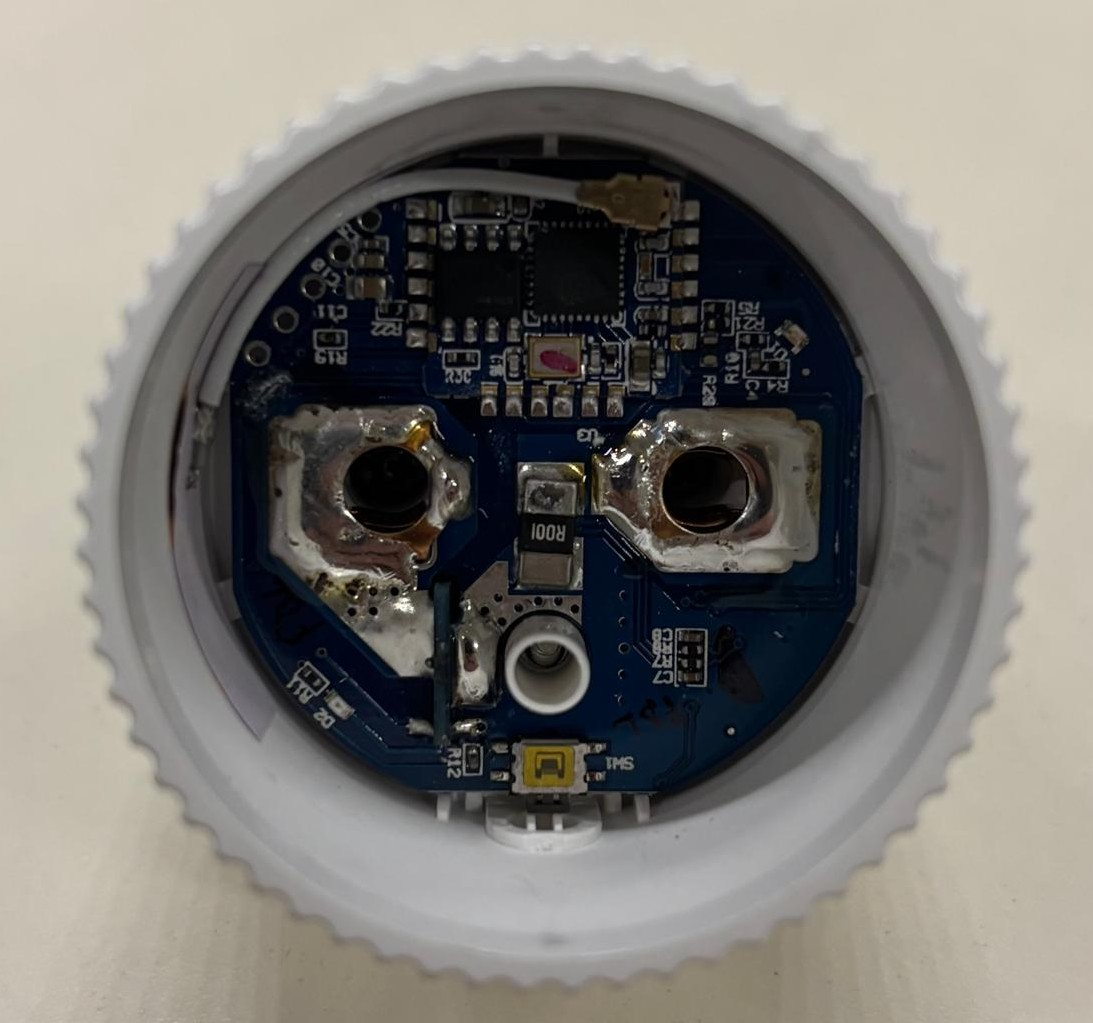
\includegraphics[width=0.4\linewidth]{Images/Fase1/Shelly Plug S Gen1 PCB.jpeg}
    \caption{Shelly Plug S PCB}
\end{figure}

\noindent The identification of these components, and in particular the combination of external memory and accessible UART interface, defines the physical attack surface of the device, enabling the vulnerability analysis and reverse engineering operations explored in this chapter.


\section{Firmware Analysis and Dumping}
Starting from the hardware configuration analyzed, this section describes the technical procedures performed to interface with the ESP8266 SoC and subsequently acquire the original firmware.

\medskip
\noindent The main goal is to establish stable serial communication to extract the binary data residing in the external flash memory.


\subsection{Identification of the UART Interface}
The first step of the analysis involved a visual inspection of the PCB. Many manufacturers leave test points exposed for factory programming or debugging; in the case of the Shelly Plug S, pinouts were identified that are accessible without the need to desolder critical components. 

\noindent Subsequently, the connection mapping between the UART test points and the SoC pins were identified using a multimeter in continuity mode.

\medskip
\noindent To establish communication between the PC and the target, ensuring data integrity and the safety of the logical components, the following instrumentation was used:

\begin{itemize}
    \item \textbf{USB-to-UART Adapter:} Specifically, a USB-to-TTL adapter was used to convert the USB signal into serial communication. It operates at TTL (Transistor-Transistor Logic) voltage levels, which were configured to 3.3V to ensure full compatibility with the SoC.
    
    \item \textbf{Jumper Cables:} The connection between the adapter and the Shelly PCB was made using Male-to-Female (M-F) jumper cables. Since the Shelly Plug S (Gen 1) features headerless test holes, it was necessary to hold the jumpers in position manually to maintain a stable signal during the dumping phase.
\end{itemize}

\begin{figure}[H]
    \centering
    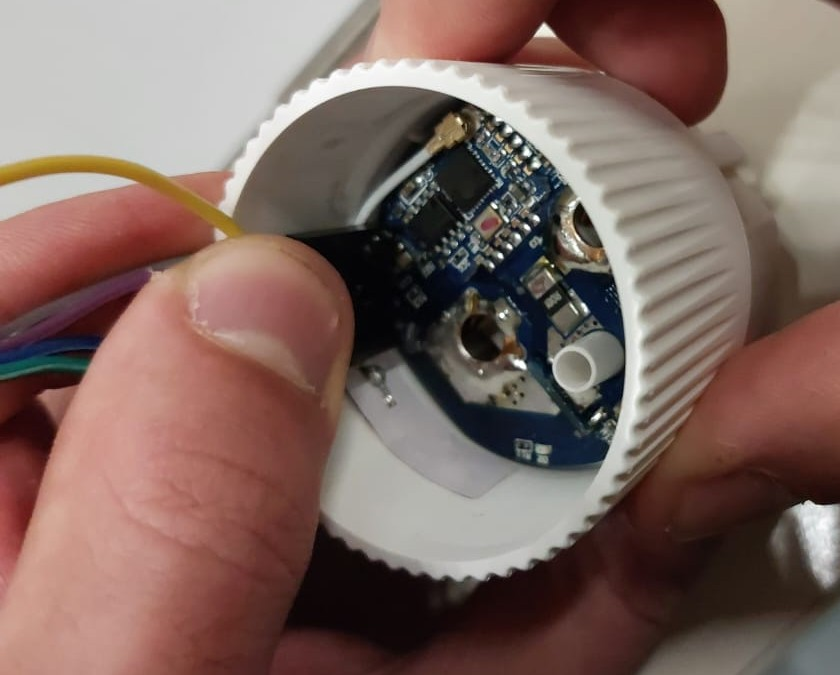
\includegraphics[width=0.4\linewidth]{Images/Fase1/foto1.jpeg}
    \caption{Jumper cables held manually in place}
\end{figure}

\noindent As indicated in the technical specifications, the ESP8266 operates in a voltage range between 2.5V and 3.6V. It was therefore essential to configure the adapter to the logical voltage of 3.3V; a higher voltage (such as 5V) would cause irreversible damage to the chip.

\medskip
\noindent The connections were made following a standard cross-over configuration:

\begin{itemize}
    \item \textbf{TX} of the Shelly to the \textbf{RX} of the adapter for transmitting data from the target to the PC.
    \item \textbf{RX} of the Shelly to the \textbf{TX} of the adapter for receiving commands sent from the PC.
    \item \textbf{GND} of the Shelly to the \textbf{GND} of the adapter to establish a common ground reference.
    \item \textbf{VCC} of the Shelly to the \textbf{VCC} of the adapter to power the chip during the operation.
\end{itemize}

\begin{figure}[H]
    \centering
    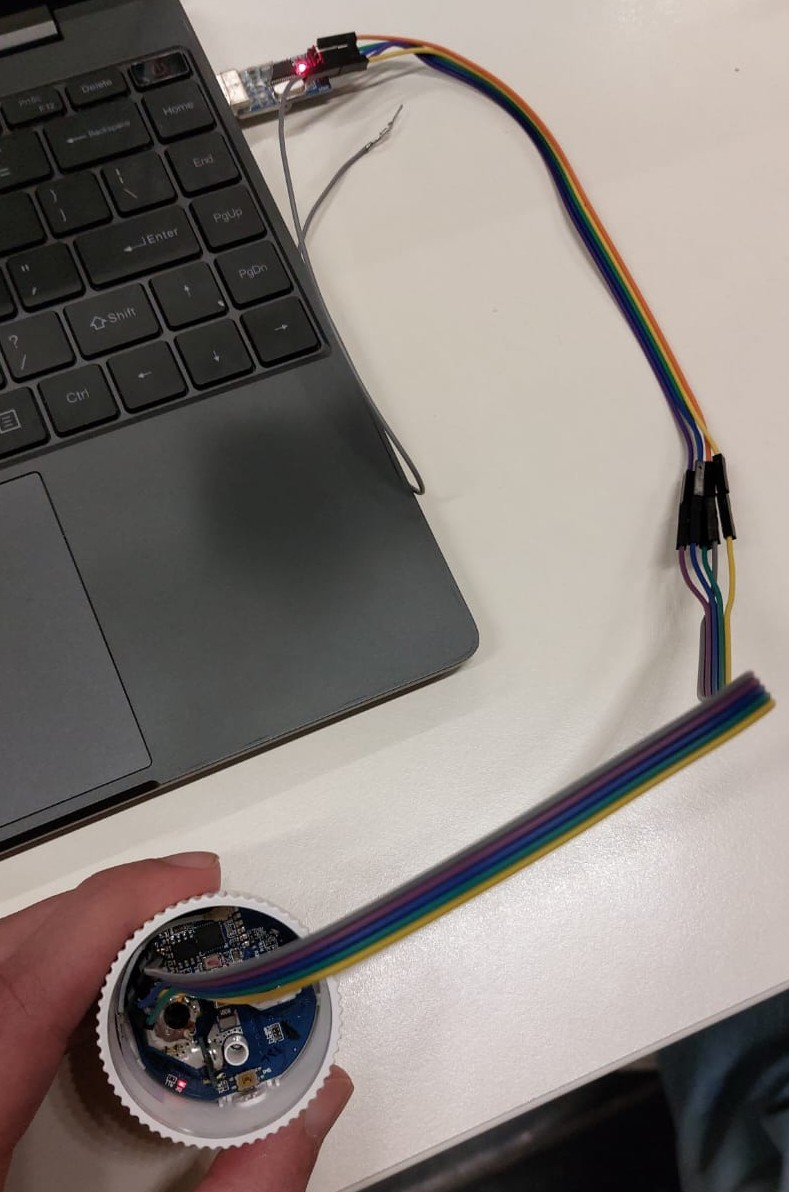
\includegraphics[width=0.4\linewidth]{Images/Fase1/linkTargetPC.jpeg}
    \caption{Communication setup between the PC and the target}
\end{figure}


\subsection{Firmware Extraction (Dumping)}
Once the physical connection is established, the extraction phase can be carried out. This operation requires coordination between the logical state of the SoC and the software interface on the PC. 

\medskip
\noindent The process consists of two steps:
\begin{enumerate}
    \item Gaining access to the download mode of the bootloader.
    \item Executing the memory read command.
\end{enumerate}

\noindent During a normal boot cycle, the ESP8266 does not allow firmware extraction; it simply executes the code present in the external flash memory. To enable memory read access via the serial interface, the chip must be forced into UART Download Mode. To achieve this, a temporary bridge was created between the GPIO0 test point and GND while connecting the USB adapter to the PC. In this state, the SoC suspends internal firmware execution and waits for serial instructions on the UART0 port.

\noindent The firmware dump was performed using esptool.py, an open-source tool specifically designed for Espressif microcontrollers. This tool enables mapping the entire address space of the external flash memory. The command executed was:

\medskip
\noindent \texttt{esptool.py --port /dev/ttyUSB0 --baud 115200 read\_flash 0 0x200000 firmware.bin}

\medskip
\noindent Where:
\begin{itemize}
    \item \texttt{--port} identifies the serial interface assigned by the operating system to the adapter (in this case, \texttt{/dev/ttyUSB0}).
    
    \item \texttt{--baud} defines the transmission speed; although the chip supports higher speeds, a standard rate of 115200 bps was chosen to ensure maximum data integrity.
    
    \item \texttt{read\_flash 0 0x200000} instructs the tool to read from address \texttt{0x0} to \texttt{0x200000} (2 MB), which matches the physical size of the flash chip.
\end{itemize}

\noindent During the dumping phase, the main challenge encountered was maintaining stable physical contact at the test points. Any minimal signal interruption on the pins caused the operation to fail, forcing a restart of the procedure. 


\subsection{Static Analysis of the Firmware}
Following the acquisition of \texttt{firmware.bin}, static analysis was performed to identify sensitive data and critical information stored in plaintext within the binary. Given the architecture of the ESP8266 SoC, which loads firmware from an external SPI flash memory at startup, the resulting file constitutes a complete image of the device software, containing the application logic, the network stack, and the configuration parameters.

\medskip
\noindent An initial analysis of the binary structure revealed that the 2 MB flash memory is divided into two symmetrical partitions of 1 MB each. This architecture is characteristic of devices supporting Over-the-Air (OTA) updates via a dual-partition scheme. This mechanism ensures redundancy: while one partition runs the active firmware, the other remains available to download and verify a new update, allowing recovery in case of write or boot errors.

\medskip
\noindent To inspect the internal structure and extract the file system, the \texttt{binwalk} tool was used with the extraction option:

\medskip
\noindent \texttt{binwalk -e firmware.bin}

\begin{figure}[H]
    \centering
    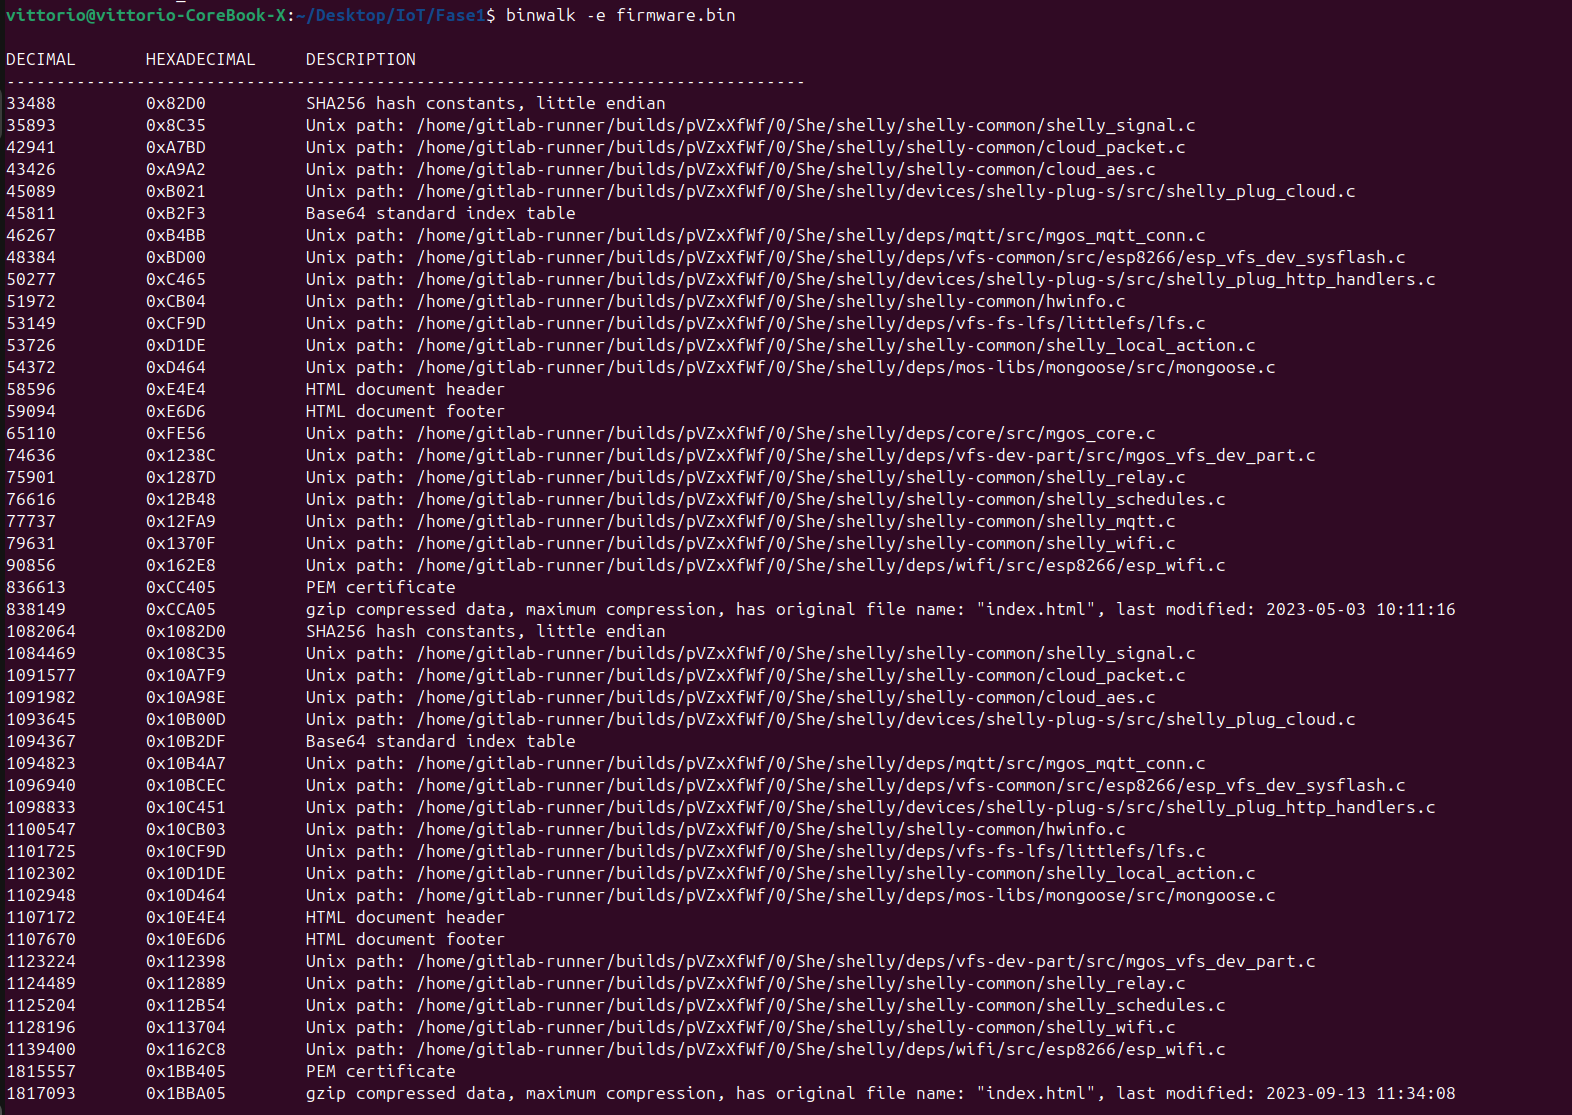
\includegraphics[width=0.95\linewidth]{Images/Fase1/binwalk -e command.png}
    \caption{Execution of the binwalk tool to extract the firmware file system}
    \label{fig:binwalk_extract}
\end{figure}

\begin{figure}[H]
    \centering
    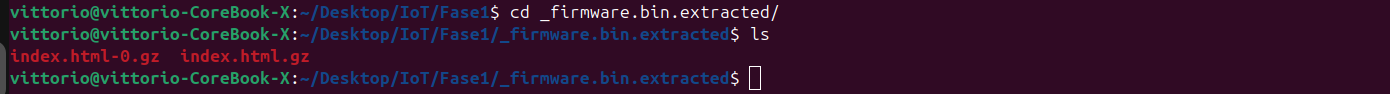
\includegraphics[width=0.85\linewidth]{Images/Fase1/cd bin extract.png}
    \caption{Contents of the extracted directory showing the web interface index.html}
    \label{fig:binwalk_dir}
\end{figure}

\noindent The analysis allowed the identification of the firmware structure and the isolation of its different sections, making them available for subsequent investigation.

\noindent Next, the list of all printable character sequences in the binary was extracted using the \texttt{strings} command. This operation allowed us to map the logical structure of the device and identify several critical pieces of information:

\begin{itemize}
    \item \textbf{Architecture and Operating System:} The analysis confirmed the use of the \textbf{ESP8266} chipset (Xtensa architecture) and the \textbf{rBoot v1.2.1} bootloader, which manages the startup and partition selection. The system is based on the \textbf{Mongoose OS v3.0.6-dev} framework, a dedicated IoT operating system. The SPI flash mode configuration was identified as \textbf{QOUT} or \textbf{DOUT}.
    
    \item \textbf{Network Credentials:} A section of the firmware, formatted as a JSON file, contains the WiFi configuration parameters in plaintext. Sensitive data such as the \textbf{SSID}, \textbf{WiFi password}, \textbf{static IP address}, and \textbf{Gateway} were successfully extracted. Storing these credentials unencrypted represents a major security vulnerability.
    
    \item \textbf{Cloud Identity and Encryption:} Unique parameters for authentication to Shelly cloud services were recovered, including the \textbf{Device ID} and the \textbf{MQTT topic} used for telemetry. Particularly critical was the discovery of static \textbf{AES keys} and their associated \textbf{Initialization Vectors (IVs)}, alongside a certificate. Because these keys are statically embedded in the firmware, the cryptographic integrity of the communications channel is compromised.
    
    \item \textbf{Source File References:} Paths to the original source code files used by Shelly developers were exposed, such as files responsible for pin mapping and low-level peripheral management.
\end{itemize}

\noindent The most significant configuration file extracted is shown below:

\begin{itemize}
    \item \textbf{Configuration file}:

\begin{verbatim}
 {
  "device": {
    "id": "shellyplug-s-DC43B6",
    "name": "Caricabatterie eskoot"
  },

  "dns_sd": {
    "host_name": "shellyplug-s-DC43B6"
  },

  "mqtt": {
    "will_topic": "shellies/shellyplug-s-DC43B6/online"
  },

  "wifi": {
    "ap": {
      "enable": false,
      "ssid": "shellyplug-s-DC43B6",
      "channel": 1,
      "hostname": "shellyplug-s-DC43B6"
    },
    "sta": {
      "enable": true,
      "ssid": "FDL",
      "pass": "fdlmj@19841987",
      "last_bssid": "b4:fb:e4:c1:d4:31",
      "last_channel": 1,
      "ip": "192.168.1.133",
      "netmask": "255.255.255.0",
      "gw": "192.168.1.1",
      "ap_roam_migrated": true
    },
    "sta_ps_mode": 2
  },

  "first_boot": false,
  "discoverable": false,

  "cloud": {
    "enabled": true,
    "aes_key": "2715d4e63bd5e0538af17f92b2b6c547",
    "aes_iv": "43ac5edf4ad75046d55b058432aaefd5"
  },

  "pin": "&2gm<{",

  "timezone": "Europe/Rome",
  "latitude": 45.51878,
  "longitude": 9.0863,

  "tz_utc_offset": 7200,
  "tz_dst": true,
  "tz_next_dst_shift": 1698541200,
  "tz_next_utc_offset": 3600,
  "tz_has_dst": 1,
  "tz_is_dst": 1,

  "wrong_sta_protect": {
    "sta_enable": true,
    "sta_ssid": "FDL",
    "sta_pass": "fdlmj@19841987"
  },

  "max_power": 200,

  "relays": {
    "r0": {
      "default_state": 2
    }
  },

  "led_status_disable": true
}

\end{verbatim}

\item \textbf{A certificate}:

\vspace{0.1cm}
\begin{verbatim}
-----BEGIN CERTIFICATE-----
MIIC+TCCAeGgAwIBAgIJAPTc08oPlcrHMA0GCSqGSIb3DQEBCwUAMBMxETAPBgNV
BAoMCEFsbHRlcmNvMB4XDTE3MDIwMzEzMjUxMFoXDTE5MTEyNDEzMjUxMFowEzER
MA8GA1UECgwIQWxsdGVyY28wggEiMA0GCSqGSIb3DQEBAQUAA4IBDwAwggEKAoIB
AQDHGDBDHpPUbtC9QAAjX3bi487A
VY5JgYB2gyp6R9cjdsNGMbYnWdxnBmsIUKJP
g7B5NcQObiMe6djUvwo0c2Xl9L+P9LOskP2WNDdpquX3XJu580hXHHVBmwOgJ0fi
+5U9mOFHhc1gYGLmhO9oqsE80SgpmsPQHloMIqmcaolLzgC9PWGu8nSDToJq+dXy
NFHzLVyBEugHQpeIR8Fq0do4dtlsfTWvv9U+fpGPegjdkPenSxGrOVwdsyFzNahx
QGKmpZE/1fsq5QSh9+Z
gwpdDChVNpkj9TBC1ApDTUasNco/6Meb/0XurpxpWPNfk
IpZ7ebtGHVd/ZkGTPUnL7FXHAgMBAAGjUDBOMB0GA1UdDgQWBBRn4Wja69QmBliB
fIg3fkettiukNDAfBgNVHSMEGDAWgBRn4Wja69QmBliBfIg3fkettiukNDAMBgNV
HRMEBTADAQH/MA0GCSqGSIb3DQEBCwUAA4IBAQBJ3GGiYs8w65ZK2bn+r6orN6Ni
FJv9r2vTxK
Arv5iSzvMky4L+8V6xBE4iCR1bfPMP/Iz8yfNEH3wStpBdyctjik8B
VX3XgiDmO0lZFRyMT6F4Z+H9obqYu3dMSGtQrfsVHqlBQVWjbXQSTmCvAQBLRym0
FT8mQ6Qt/bvb2F2y1QtFhHWqUnjiwWui5F2+hb2xJdI80QSI1v0tw4V0IaOHcPQT
3QAyDHujNhZGfeY9m8vJFfEDe2JvMx+wp27V5AyRMO0nfk8yJDSUSBXLpkH6ExkH
aUta9TCY9Mg7vLEmM7H2LTrVawi1PrZj2gEdkEZL/9r2H1PAN7NQtpG9Mur
-----END CERTIFICATE-----
    \end{verbatim}

\item \textbf{Encryptions informatons}:

\begin{verbatim}
/home/gitlab-runner/builds/pVZxXfWf/0/She/shelly/shelly-common/cloud_aes.c
aes-internal-enc.c
  { "aes_key": "403d3d45f9b96ced81a98f032def693e",
    "aes_iv": "b811c906d70565e9bdc83cff3ca38605"},
  
  { "aes_key": "a54cee7a138a1f1e22819fb65911daa3",
    "aes_iv": "7b9d3cabcfb872e1bb25938548b7a494"},
  
  { "aes_key": "93b5f30271bf18c993e0b2a6dc0b1cd4",
    "aes_iv": "33df99be201a2326ef4a156eb3cfcf2c"},
  
  { "aes_key": "a8c1b8a705c8aa7c6d24",
    "aes_iv": "961f0a10417c1a2afaa610d880c2ca25"},
  
  { "aes_key": "720108495d63cba66274b7ae4bbbab74",
    "aes_iv": "38c7875e8d8fc9da88c925c129afba43"},
  
  { "aes_key": "c173df474b63656ba425be6975ec7e93",
    "aes_iv": "1d18a320e650fbfe141d208bfbbba68b"},
  
  { "aes_key": "2715d4e63bd5e0538af17f92b2b6c547",
    "aes_iv": "43ac5edf4ad75046d55b058432aaefd5"},
  
  { "aes_key": "4698d73b194a6bf75a97630c44a84820",
    "aes_iv": "46ed6177ff2330f4ac5e6be2ff6b36c0"},
  
  { "aes_key": "3c72611edcb5ba37bc455e7e74df2e6a",
    "aes_iv": "1f12d9366b8c1651f5a22bd830db0930"},
    
  { "aes_key": "177bdd5d99619613457a6181f134df02",
    "aes_iv": "f2b9426382aa54966f0c3e18d7bf28d7"},
    
  { "aes_key": "cb337b24d69fc3871eaacccaa668237f",
    "aes_iv": "83f8ce5bbd013296fab61fd18abe372f"},
  
  { "aes_key": "ea5822e253ab96772b9b590de3ac275e",
    "aes_iv": "793c6e9aa4c87662f91c6d9fe2eab64f"},
    
  { "aes_key": "6545bef05ffbb37bf0b27e2b15823fd8",
    "aes_iv": "a08203b539f59caf17b2f4df06ee8a02"},
  
  { "aes_key": "c7fca300f90c50983beecd46f3a986fc",
    "aes_iv": "9815c9253358cbe7bbaba6b7f0e4aa9a"},
    
  { "aes_key": "23553ebc700e8d60f143bbfcecce1b27",
    "aes_iv": "963da4a27a9045a5b57fcaeecc9968ae"},

  { "aes_key": "8025d668363f2ab4b6d0896410a9d4a5",
    "aes_iv": "aa8fbf160ac9c9f997388e4b28edc85b"}
  
\end{verbatim}

\item \textbf{Important URL's used}:

\begin{verbatim}
http://api.shelly.cloud/files/firmware
http://api.shelly.cloud/timezone/autodetect?time=%ld&fw=%s
http://api.shelly.cloud/timezone/tzinfo?tz=%s&time=%ld&fw=%s
\end{verbatim}

\end{itemize}

\noindent The most significant result of the static analysis was the identification of the official OTA update URL endpoint: \url{http://api.shelly.cloud/files/firmware}. Accessing this endpoint returned a JSON-formatted list containing references to all firmware releases for the various Shelly device models. This discovery is crucial for the next phase of the project, as it identifies the exact target for a Man-in-the-Middle (MITM) attack.

\begin{figure}[H]
    \centering
    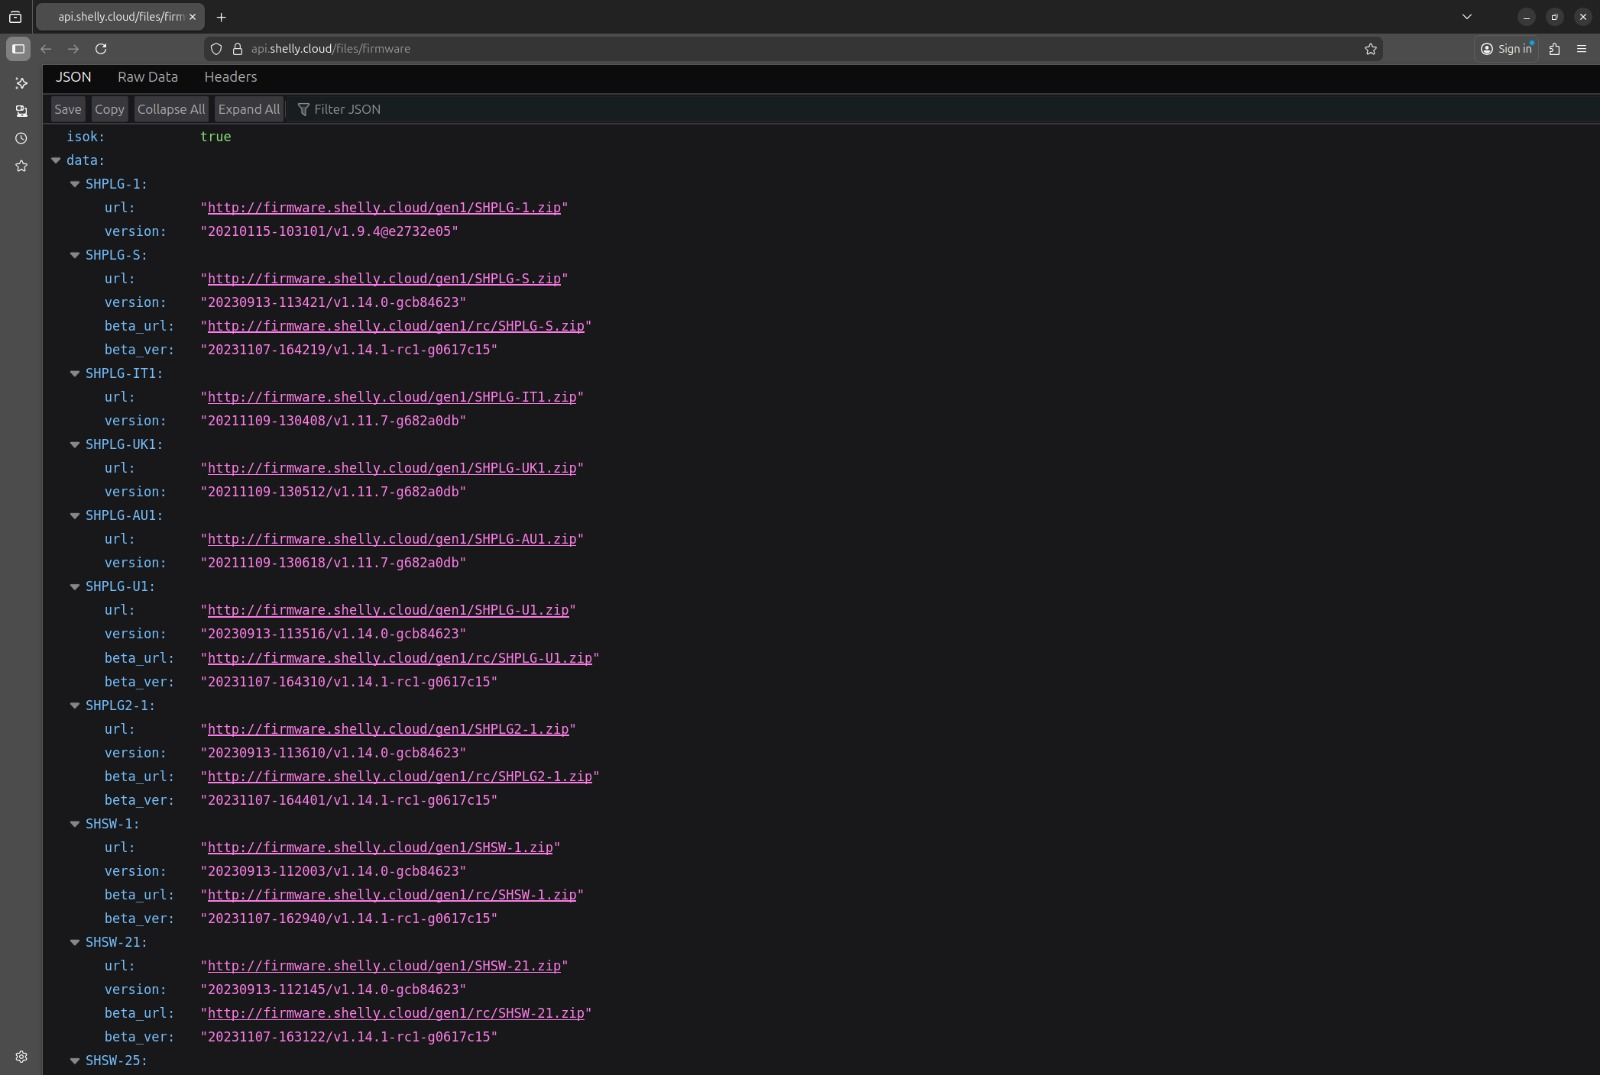
\includegraphics[width=0.95\linewidth]{Images/Fase1/url list.jpeg}
    \caption{GET result of the official firmware list endpoint}
    \label{fig:url_firmware_list}
\end{figure}


\subsection{Analysis of the OTA Update Mechanism}
The OTA (Over-the-Air) update mechanism of the Shelly Plug S (Gen 1) relies entirely on unencrypted HTTP communication. When a firmware update is initiated—either by the user through the local web interface or automatically via the cloud—the device sends an HTTP GET request to retrieve the binary file from the specified URL.

\noindent During this process, the device establishes a TCP connection over port 80 without any transport-layer encryption (SSL/TLS). Once the binary is downloaded, the bootloader writes the incoming data directly to the inactive flash partition. 

\noindent Crucially, the original firmware does not perform any cryptographic verification (such as digital signatures or public-key validation) to confirm the authenticity and integrity of the downloaded binary. The device only performs basic structural checks (magic bytes and checksum validation) on the ESP8266 image headers before swapping the active partition and rebooting. This complete lack of cryptographic signature verification allows an attacker to inject arbitrary binaries simply by intercepting the HTTP request and redirecting it to a server hosting a modified image, which is the exploit demonstrated in Phase 2.


\section{MQTT: Insecure Protocol Demonstration}
The original factory firmware of the Shelly Plug S relies on standard, unencrypted MQTT over TCP port 1883 for local communication and integration with home automation platforms. In this default configuration, all telemetry data—including real-time power consumption, voltage, and relay status—is transmitted across the network in plaintext. Similarly, control commands (such as switching the relay on or off) are sent without encryption or session authentication.

\noindent In the original firmware settings, MQTT can only be enabled under the "Advanced - Developer Settings" menu. As shown in Figure~\ref{fig:shelly_net_sec} and Figure~\ref{fig:shelly_mqtt_config}, the configuration parameters are limited to the broker's IP address, username, and password. There is no option to enable SSL/TLS encryption or configure client certificates for mutual authentication.

\begin{figure}[H]
    \centering
    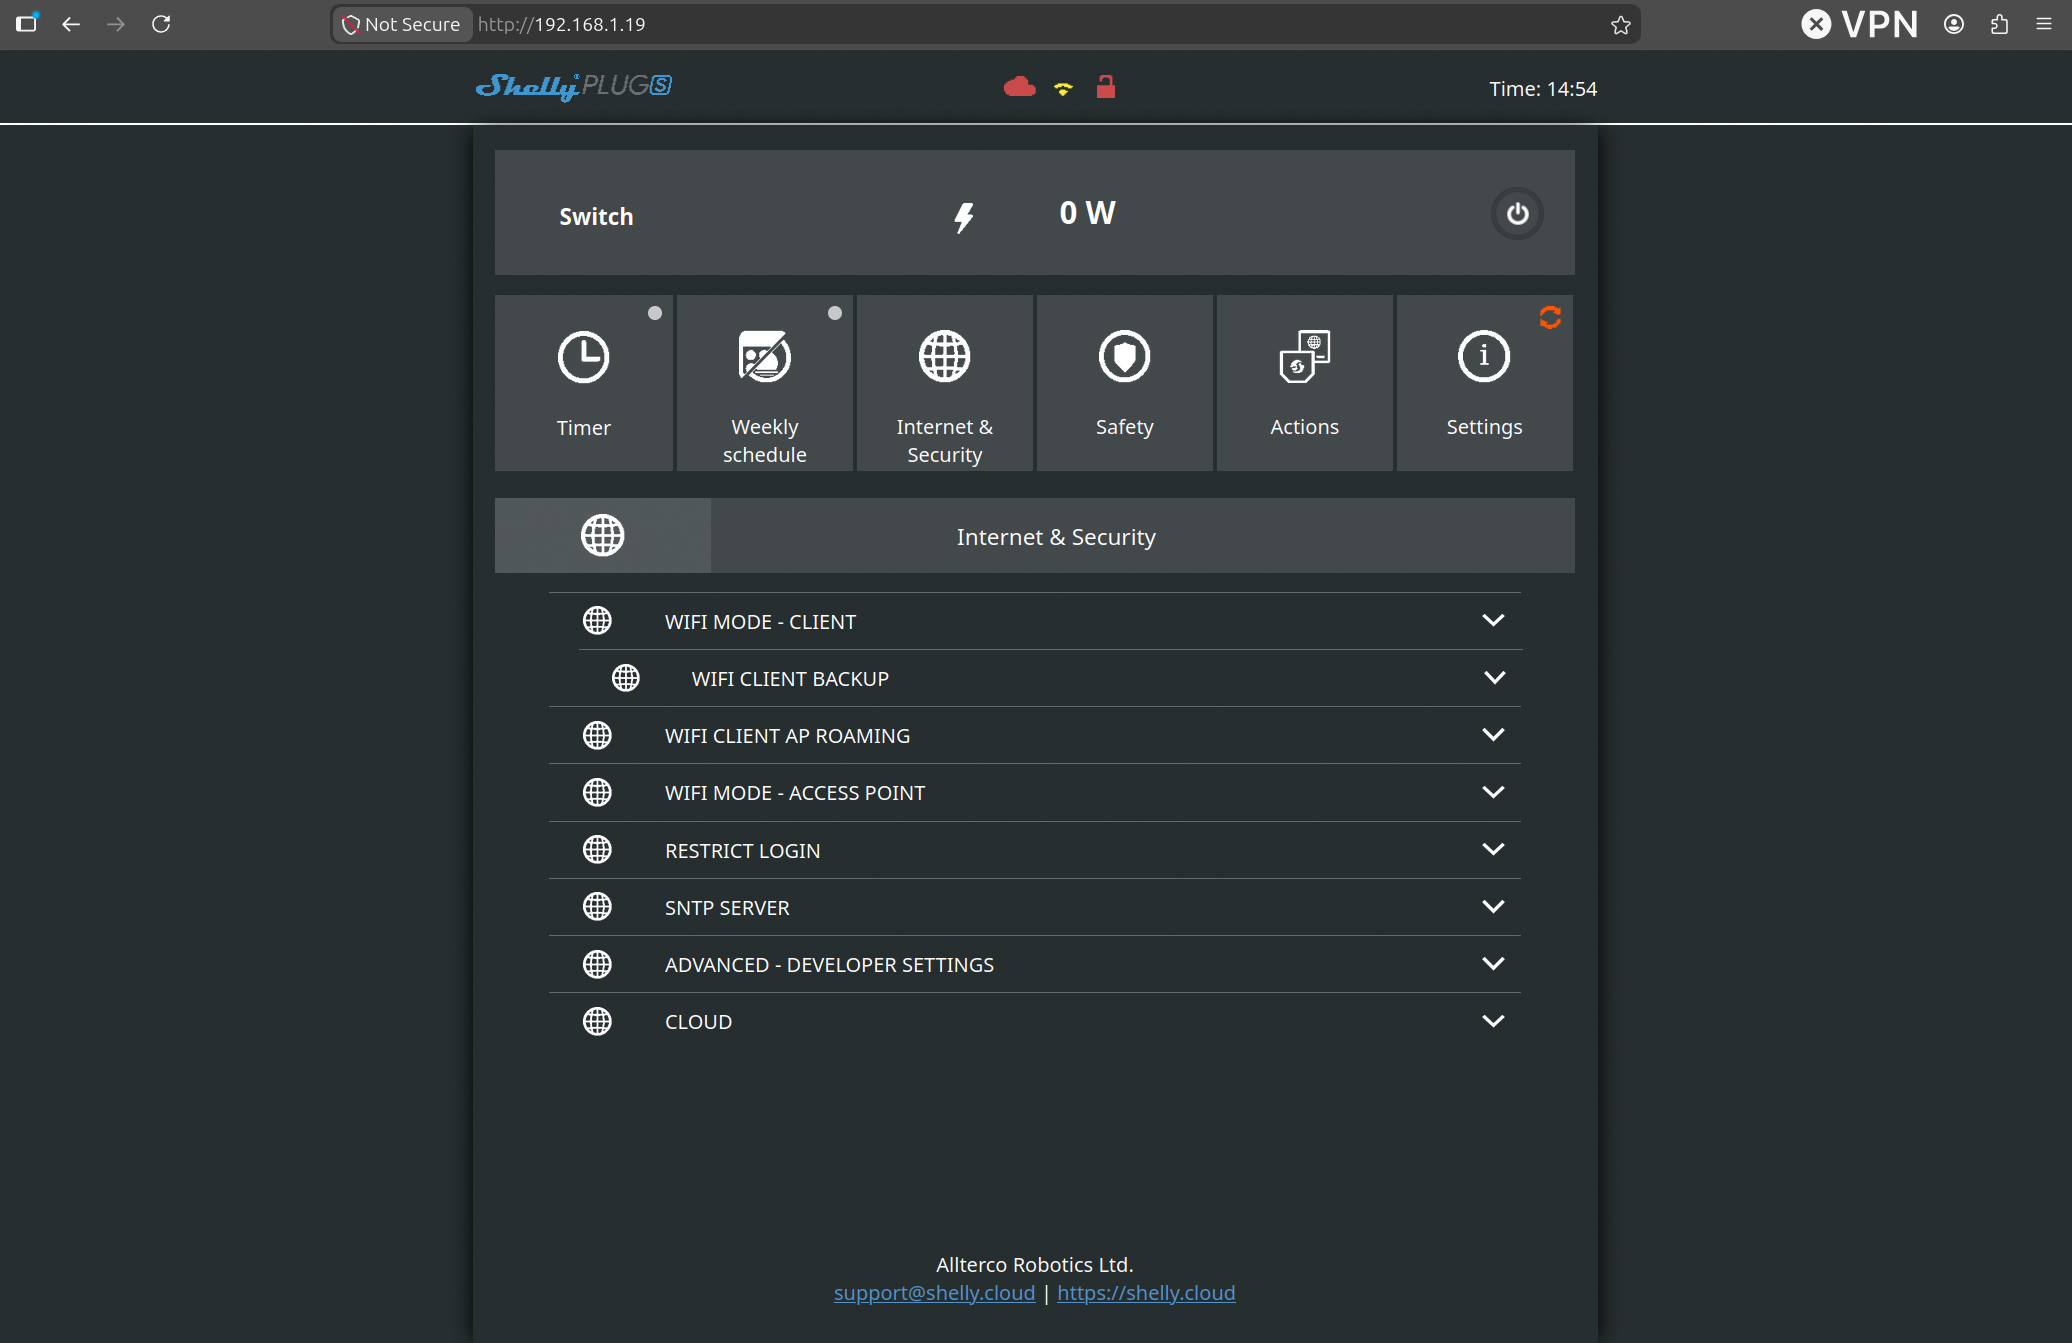
\includegraphics[width=0.9\linewidth]{Images/Fase1/Interfaccia3.png}
    \caption{Internet \& Security settings menu in the local Web UI}
    \label{fig:shelly_net_sec}
\end{figure}

\begin{figure}[H]
    \centering
    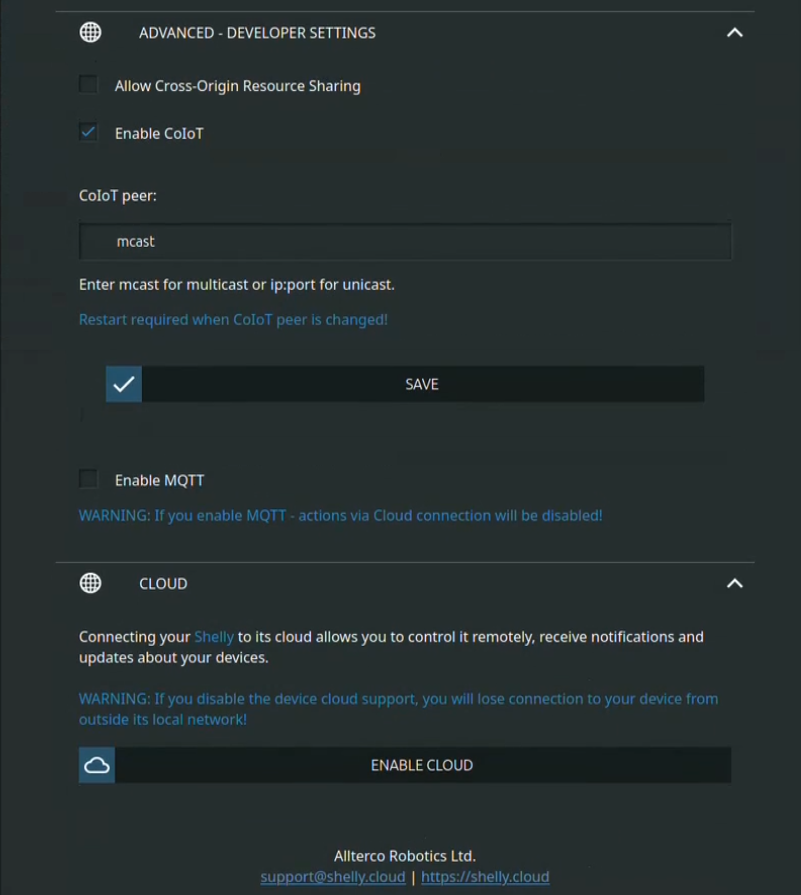
\includegraphics[width=0.5\linewidth]{Images/Fase1/Interfaccia6.png}
    \caption{Advanced Developer Settings demonstrating the lack of MQTT encryption options}
    \label{fig:shelly_mqtt_config}
\end{figure}

\noindent To demonstrate this protocol vulnerability, a local traffic capture was performed using Wireshark on TCP port 1883. Since the communication is completely unencrypted, an attacker on the local network can intercept the telemetry topics in cleartext.

\noindent As shown in Figure~\ref{fig:wireshark_power}, the real-time active power consumption is transmitted in plaintext under the \texttt{relay/0/power} topic (capturing a payload of 11.78 W).

\begin{figure}[H]
    \centering
    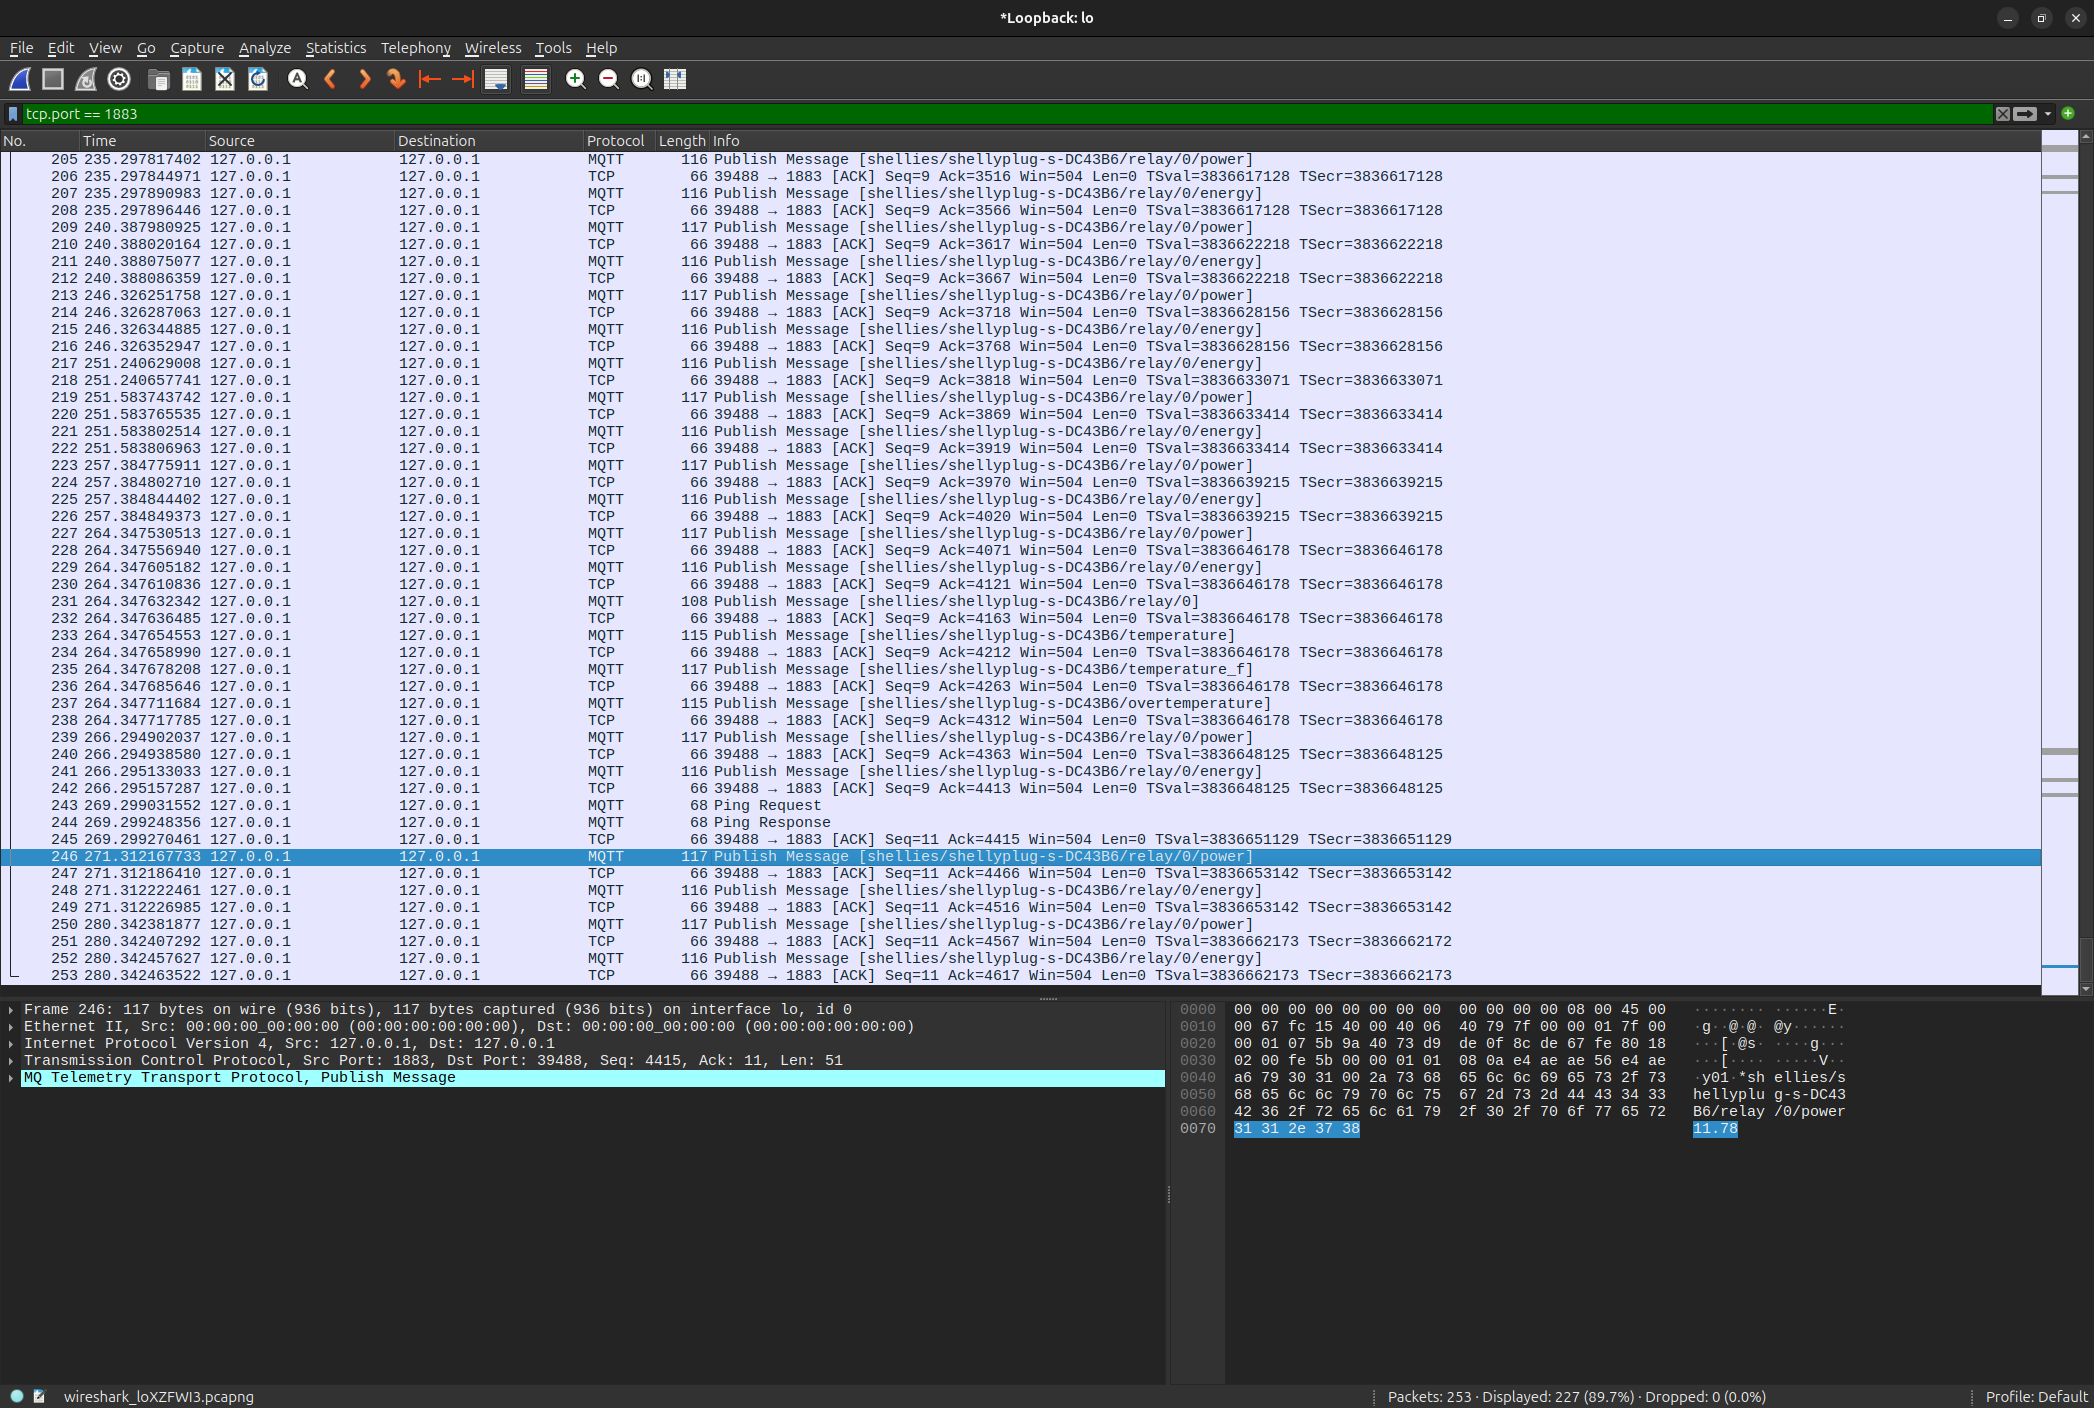
\includegraphics[width=0.8\linewidth]{Images/Fase1/MQTT1.png}
    \caption{Sniffed MQTT packet showing active power consumption in plaintext}
    \label{fig:wireshark_power}
\end{figure}

\noindent Similarly, cumulative energy values are exposed under the \texttt{relay/0/energy} topic (Figure~\ref{fig:wireshark_energy}), while the physical state of the relay (on/off) can be monitored in real time on the \texttt{relay/0} topic (Figure~\ref{fig:wireshark_state}).

\begin{figure}[H]
    \centering
    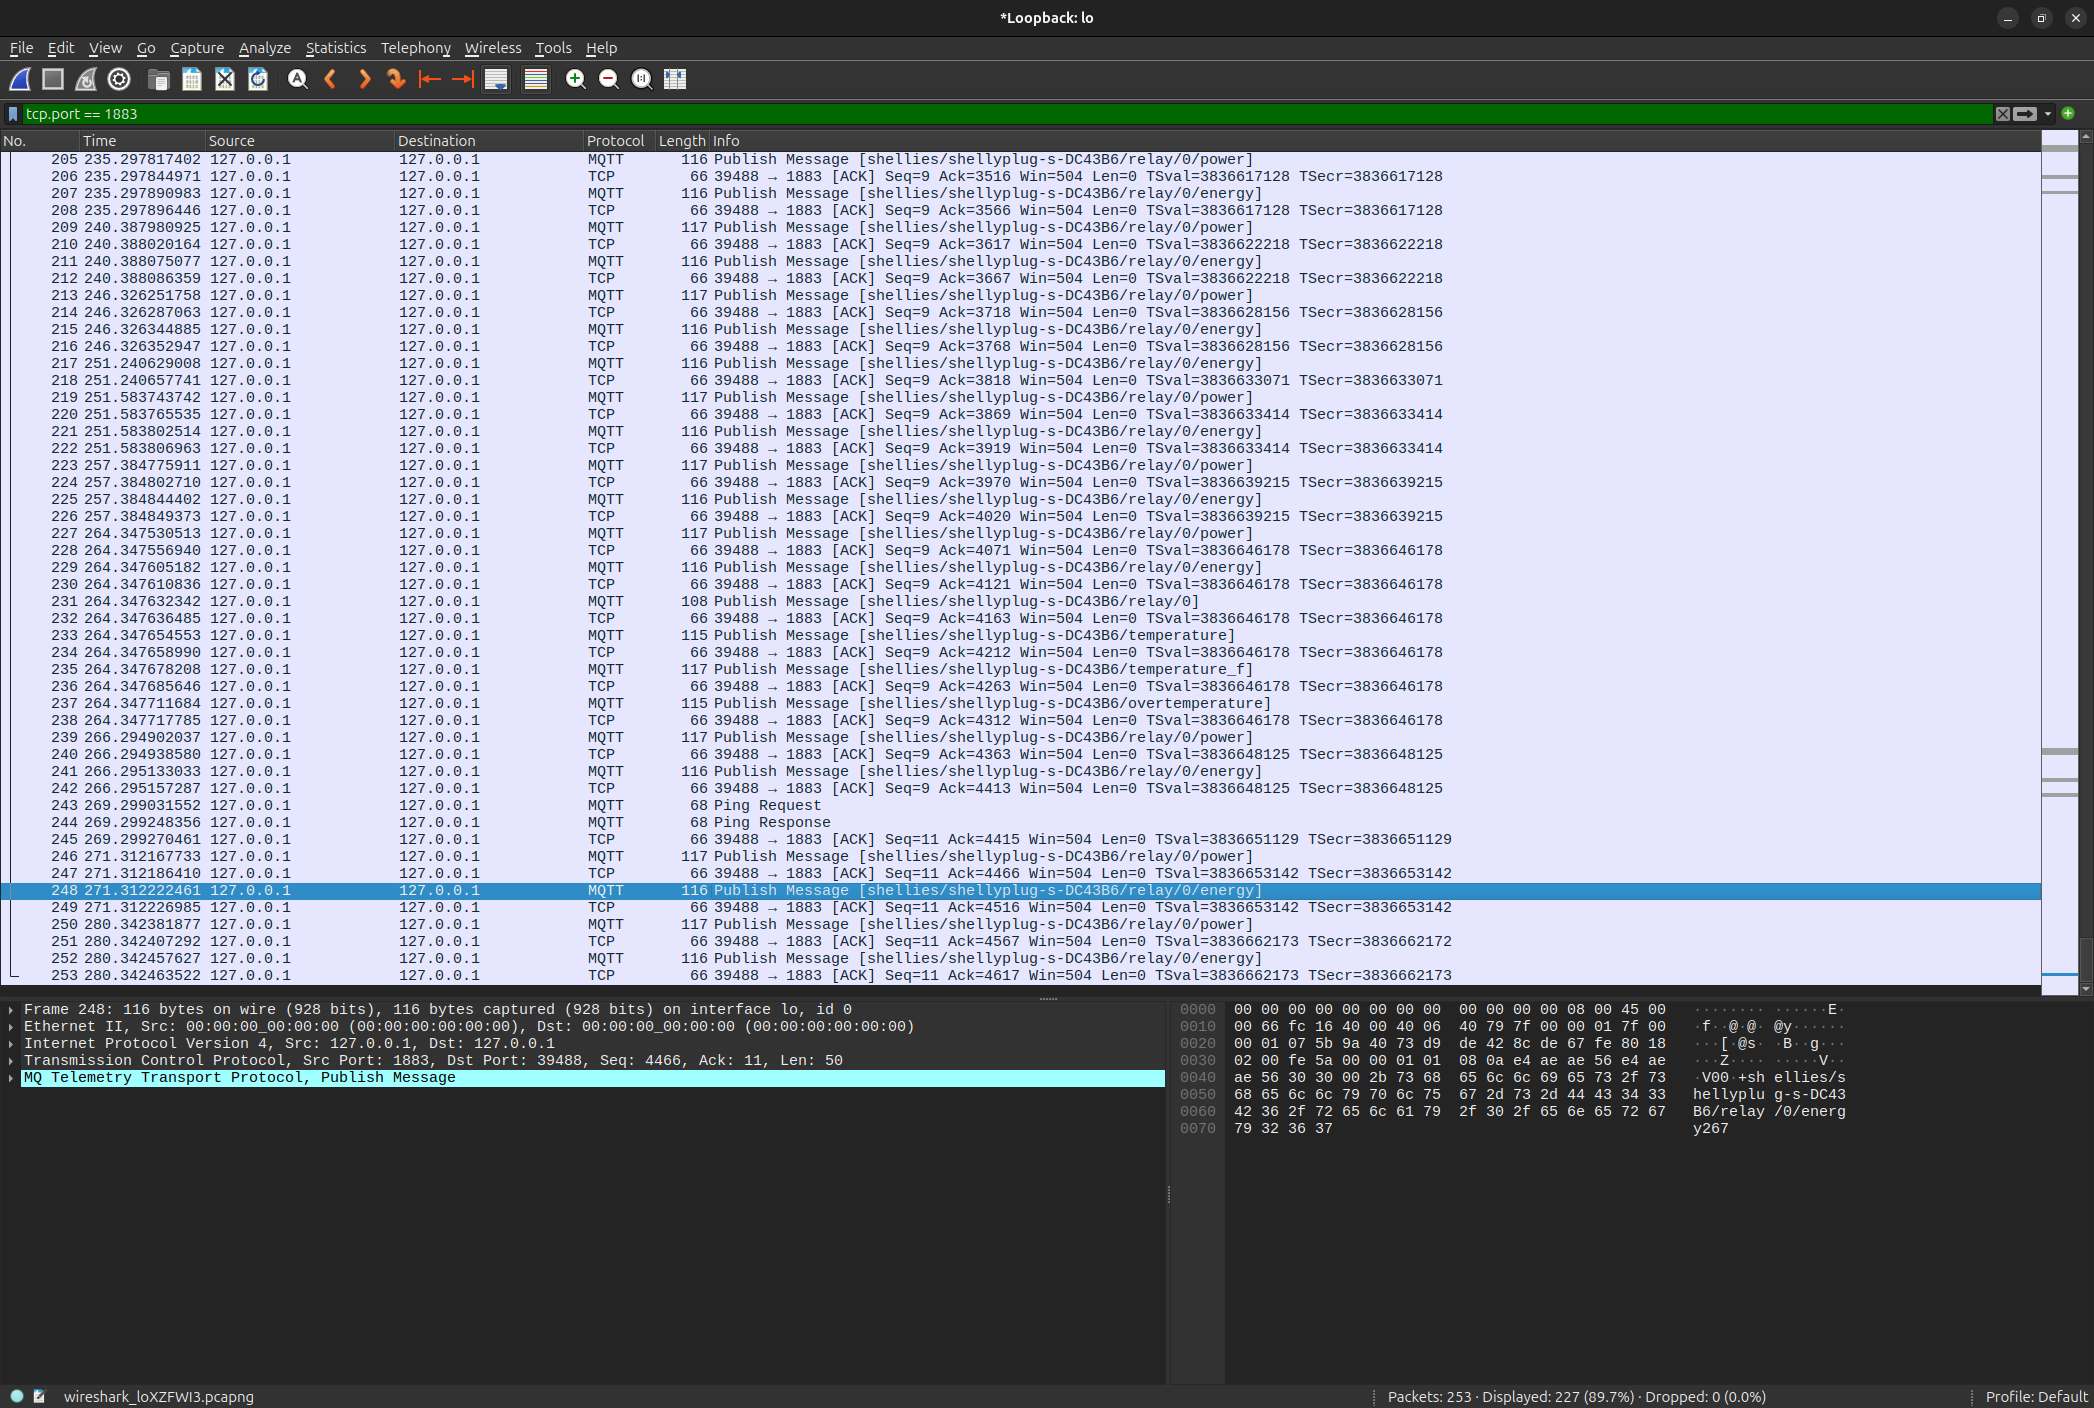
\includegraphics[width=0.8\linewidth]{Images/Fase1/MQTT2.png}
    \caption{Sniffed MQTT packet showing cumulative energy in plaintext}
    \label{fig:wireshark_energy}
\end{figure}

\begin{figure}[H]
    \centering
    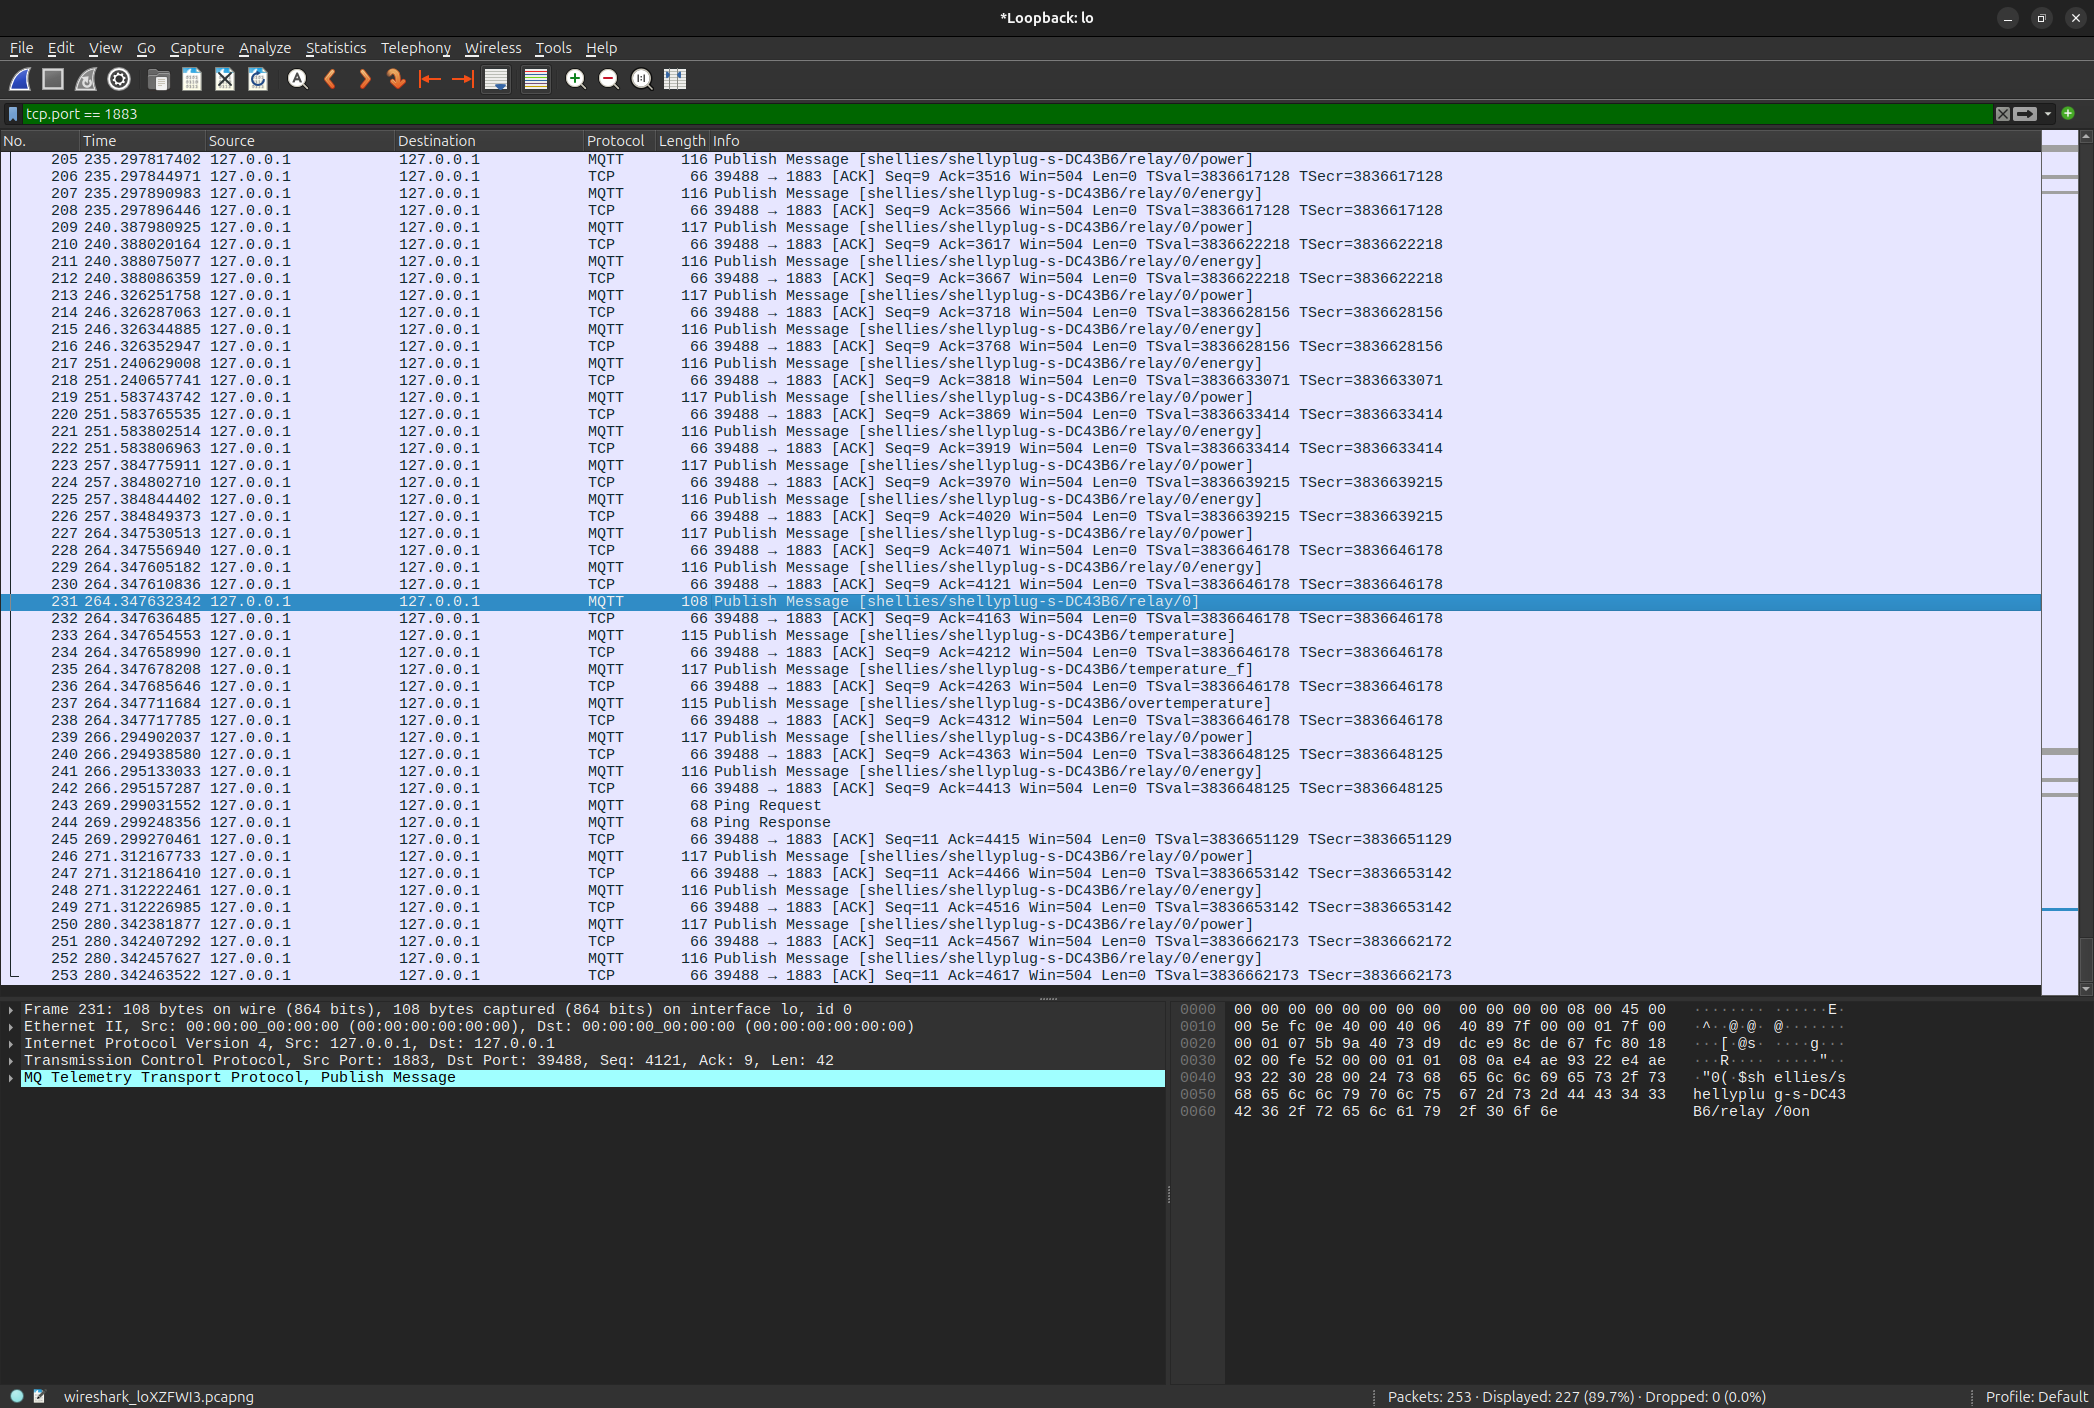
\includegraphics[width=0.8\linewidth]{Images/Fase1/MQTT3.png}
    \caption{Sniffed MQTT packet showing the relay state command ("on") in plaintext}
    \label{fig:wireshark_state}
\end{figure}

\noindent Crucially, the factory firmware does not support MQTT over TLS (MQTTS) or mutual authentication (mTLS) with client certificates. This limitation is primarily due to the design choices of the original firmware, which prioritized lightweight protocols over transport security to minimize RAM consumption on the ESP8266. This protocol insecurity leaves the local communication channel entirely exposed to sniffing and unauthorized command injection, highlighting the need for the hardening countermeasures implemented in Phase 3.


\section{Threat Modeling}
Based on the physical and protocol analysis performed in this phase, the following STRIDE matrix maps the identified vulnerabilities, the potential exploitation vectors (demonstrated in Phase 2), and the proposed countermeasures implemented in Phase 3.

\begingroup
\footnotesize
\renewcommand{\arraystretch}{1.3}
\setlength{\tabcolsep}{4pt} % Riduce la spaziatura interna tra colonne per evitare sforamenti
\begin{longtable}{>{\raggedright\arraybackslash}p{0.12\textwidth} >{\raggedright\arraybackslash}p{0.22\textwidth} >{\raggedright\arraybackslash}p{0.29\textwidth} >{\raggedright\arraybackslash}p{0.29\textwidth}}
\caption{Threat Modeling and STRIDE Matrix for Shelly Plug S Gen 1} \label{tab:stride_matrix} \\
\toprule
\textbf{\color{darkblue}Category} & \textbf{\color{darkblue}Description} & \textbf{\color{darkblue}Shelly Gen1 Scenario (Fase 2)} & \textbf{\color{darkblue}Mitigation Strategy (Fase 3)} \\
\midrule
\endfirsthead

\multicolumn{4}{c}%
{{\bfseries \tablename\ \thetable{} -- Continued from previous page}} \\
\toprule
\textbf{\color{darkblue}Category} & \textbf{\color{darkblue}Description} & \textbf{\color{darkblue}Shelly Gen1 Scenario} & \textbf{\color{darkblue}Mitigation Strategy (Fase 3)} \\
\midrule
\endhead

\bottomrule
\endfoot

\bottomrule
\endlastfoot

\rowcolor{lightgray}
\textbf{S}poofing & Impersonating a client, broker, or update server. & [\textbf{Implemented}] MITM attack redirecting the device to a rogue OTA update server serving a fake manifest. & \textbf{[Implemented]} Mutual TLS (mTLS) with ECC certificates for broker identity; RSA signatures for firmware source validation. \\
\addlinespace
\textbf{T}ampering & Unauthorized modification of code or telemetry data. & [\textbf{Implemented}] Injecting custom Mongoose OS firmware via unsigned OTA binaries. & \textbf{[Implemented]} Secure OTA update verifying RSA-2048 / SHA-256 firmware signatures using BearSSL. \\
\addlinespace
\rowcolor{lightgray}
\textbf{R}epudiation & Inability to audit or trace actions and commands. & \textit{[Out of Scope]} Triggering relay actions via unauthenticated local HTTP or MQTT commands with no audit log. & \textit{[Out of Scope]} Logging unique client certificate CN/IDs at the Mosquitto broker level. \\
\addlinespace
\textbf{I}nformation Disc. & Eavesdropping or intercepting private data. & [\textbf{Implemented}] Sniffing cleartext MQTT topics on port 1883 to leak power, energy, and relay states. & \textbf{[Implemented]} MQTTS (MQTT over TLS 1.2, port 8883) with client-side ECC encryption. \\
\addlinespace
\rowcolor{lightgray}
\textbf{D}enial of Service & Overloading resources to disrupt service. & \textit{[Out of Scope]} Flooding unauthenticated local HTTP endpoints (/relay, /reboot) to crash the ESP8266. & \textit{[Out of Scope]} Dedicated IoT VLAN segmentation and network rate-limiting rules. \\
\addlinespace
\textbf{E}levation of Priv. & Gaining unauthorized physical or logical access. & [\textbf{Implemented}] Accessing PCB UART test points to execute an esptool.py flash memory dump. & \textit{[Theoretical]} Disabling ESP8266 UART RX/TX boot modes in code and blowing chip fuses. \\
\end{longtable}
\endgroup

